\documentclass[a4paper,14pt]{extarticle}
\usepackage{fontspec}
\defaultfontfeatures[Liberation Serif]{Path={/Users/albertosipov/.cache/codex-runtimes/codex-primary-runtime/dependencies/native/libreoffice-headless/libreoffice/LibreOfficeDev.app/Contents/Resources/fonts/truetype/},UprightFont=LiberationSerif-Regular.ttf,BoldFont=LiberationSerif-Bold.ttf,ItalicFont=LiberationSerif-Italic.ttf,BoldItalicFont=LiberationSerif-BoldItalic.ttf}
\defaultfontfeatures[Liberation Sans]{Path={/Users/albertosipov/.cache/codex-runtimes/codex-primary-runtime/dependencies/native/libreoffice-headless/libreoffice/LibreOfficeDev.app/Contents/Resources/fonts/truetype/},UprightFont=LiberationSans-Regular.ttf,BoldFont=LiberationSans-Bold.ttf,ItalicFont=LiberationSans-Italic.ttf,BoldItalicFont=LiberationSans-BoldItalic.ttf}
\defaultfontfeatures[DejaVu Sans Mono]{Path={/Users/albertosipov/.cache/codex-runtimes/codex-primary-runtime/dependencies/native/libreoffice-headless/libreoffice/LibreOfficeDev.app/Contents/Resources/fonts/truetype/},UprightFont=DejaVuSansMono.ttf,BoldFont=DejaVuSansMono-Bold.ttf,ItalicFont=DejaVuSansMono-Oblique.ttf,BoldItalicFont=DejaVuSansMono-BoldOblique.ttf}
\usepackage{amsmath,amssymb,mathtools}
\usepackage{unicode-math}
\let\reportsetmathfont\setmathfont
\renewcommand{\setmathfont}[1]{\reportsetmathfont[Path={/Users/albertosipov/.cache/codex-runtimes/codex-primary-runtime/dependencies/native/libreoffice-headless/libreoffice/LibreOfficeDev.app/Contents/Resources/fonts/truetype/}]{DejaVuMathTeXGyre.ttf}}

\usepackage{../../../template/gostreport}
\ifdefined\reportsetmathfont\let\setmathfont\reportsetmathfont\fi
\usepackage{adjustbox}
\usepackage{etoolbox}
\usepackage{fvextra}
\hypersetup{pdftitle={ЛР3 — Матрицы в 3D-графике. Задания 1–5},pdfauthor={Осипов А. П.; Глазков В. Н.; Прохоревич И. Б.}}
\begin{document}
\makegosttitle{3}{Матрицы в 3D-графике}
{студент группы R3243 Осипов А.\,П.\\[4pt]
студент группы R3281 Глазков В.\,Н.\\[4pt]
студент группы R3235 Прохоревич И.\,Б.\\[8pt]
Промежуточная версия: задания 1--5}{Догадин Е.\,В.}
\tableofcontents
\clearpage
\unnumsection{Введение}
В отчёте представлены задания 1--5 лабораторной работы №3: отрисовка фигур
в однородных координатах, масштабирование, перенос и вращение куба,
сравнение порядка применения преобразований, поворот вокруг оси через вершину.
Расчёты выполнены на Python с использованием NumPy, Matplotlib и SciPy.
Все преобразования координат реализованы умножением на матрицы.
Задания 6--7 о камере и перспективе в этой версии ещё не представлены.
\unnumsection{Исходные данные}
\begin{itemize}
\item Исходный куб из методички: координаты вершин по каждой оси равны $-1$ или $1$,
  длина ребра — $2$.
\item Вершины тетраэдра, выбранные Альбертом:
  $A=(-2,-2,0)$, $B=(4,-4,0)$, $C=(0,8,0)$, $D=(1,1,10)$.
\item Коэффициенты масштабирования, выбранные Альбертом для задания 2:
  $(s_{1x},s_{1y},s_{1z})=(2,4,10)$ и
  $(s_{2x},s_{2y},s_{2z})=(0.5,1,0.1)$.
\item Векторы переноса, выбранные Альбертом для задания 3:
  $t_1=(5,5,2)$ и $t_2=(0,3,10)$.
\item Для сравнения порядка преобразований используются $T=T_1$ и $S=S_1$.
\end{itemize}
\clearpage
\section{Задание 1. Отрисовка куба и другой фигуры}

\subsection*{Однородные координаты и устройство кода}

Каждая вершина хранится в столбце матрицы \texttt{vertices} как
$\widetilde p=(x,y,z,w)^T$. Для выбранных исходных фигур $w=1$.
Переход к декартовым координатам при $w\ne0$ имеет вид

\begin{center}\adjustbox{max width=\linewidth}{$\displaystyle p=\begin{pmatrix}x/w\\y/w\\z/w\end{pmatrix}.$}\end{center}

Например, $(4,6,2,2)^T$ задаёт точку $(2,3,1)^T$.
Строка программы

\begin{lstlisting}[style=py,numbers=none]
points = (vertices[:3, :] / vertices[3, :]).T
\end{lstlisting}

выполняет это деление для всех вершин. Транспонирование \texttt{.T} переводит
матрицу размера $3\times N$ в $N\times3$: отрисовщику нужны вершины по строкам.
Каждая строка \texttt{faces} задаёт индексы вершин одной грани в порядке обхода.
Индексация начинается с нуля. \texttt{points[faces]} собирает координаты граней,
а \texttt{Poly3DCollection} отображает их в пространстве.
Использована ортографическая проекция \texttt{proj\_type="ortho"}.

\subsection*{Исходный куб}

Матрицы из Python-листинга методички:

\begin{center}\adjustbox{max width=\linewidth}{$\displaystyle V=\begin{pmatrix}
-1&1&1&-1&-1&1&1&-1\\
-1&-1&1&1&-1&-1&1&1\\
-1&-1&-1&-1&1&1&1&1\\
1&1&1&1&1&1&1&1
\end{pmatrix},$}\end{center}

\begin{center}\adjustbox{max width=\linewidth}{$\displaystyle F=\begin{pmatrix}
0&1&5&4\\
1&2&6&5\\
2&3&7&6\\
3&0&4&7\\
0&1&2&3\\
4&5&6&7
\end{pmatrix}.$}\end{center}

У грани $[0,1,2,3]$ все вершины имеют $z=-1$: это нижняя грань куба.
Центр куба находится в начале координат, длина ребра равна $2$.

\subsection*{Тетраэдр}

Вместо куба заданы вершины
$A=(-2,-2,0)$, $B=(4,-4,0)$, $C=(0,8,0)$, $D=(1,1,10)$:

\begin{center}\adjustbox{max width=\linewidth}{$\displaystyle V_{\mathrm{tetra}}=\begin{pmatrix}
-2&4&0&1\\
-2&-4&8&1\\
0&0&0&10\\
1&1&1&1
\end{pmatrix},\qquad
F_{\mathrm{tetra}}=\begin{pmatrix}
0&2&1\\
0&1&3\\
1&2&3\\
2&0&3
\end{pmatrix}.$}\end{center}

Первые три вершины лежат в плоскости $z=0$, четвёртая — вне этой плоскости.
Вместо шести четырёхугольных граней получены четыре треугольные.
Пределы осей расширены под выбранные координаты; пропорции области построения
согласованы с диапазонами осей, чтобы единичный масштаб по всем осям совпадал.
Куб и тетраэдр показаны на рисунке~\ref{fig:p01_figures}.

\begin{figure}[H]
\centering
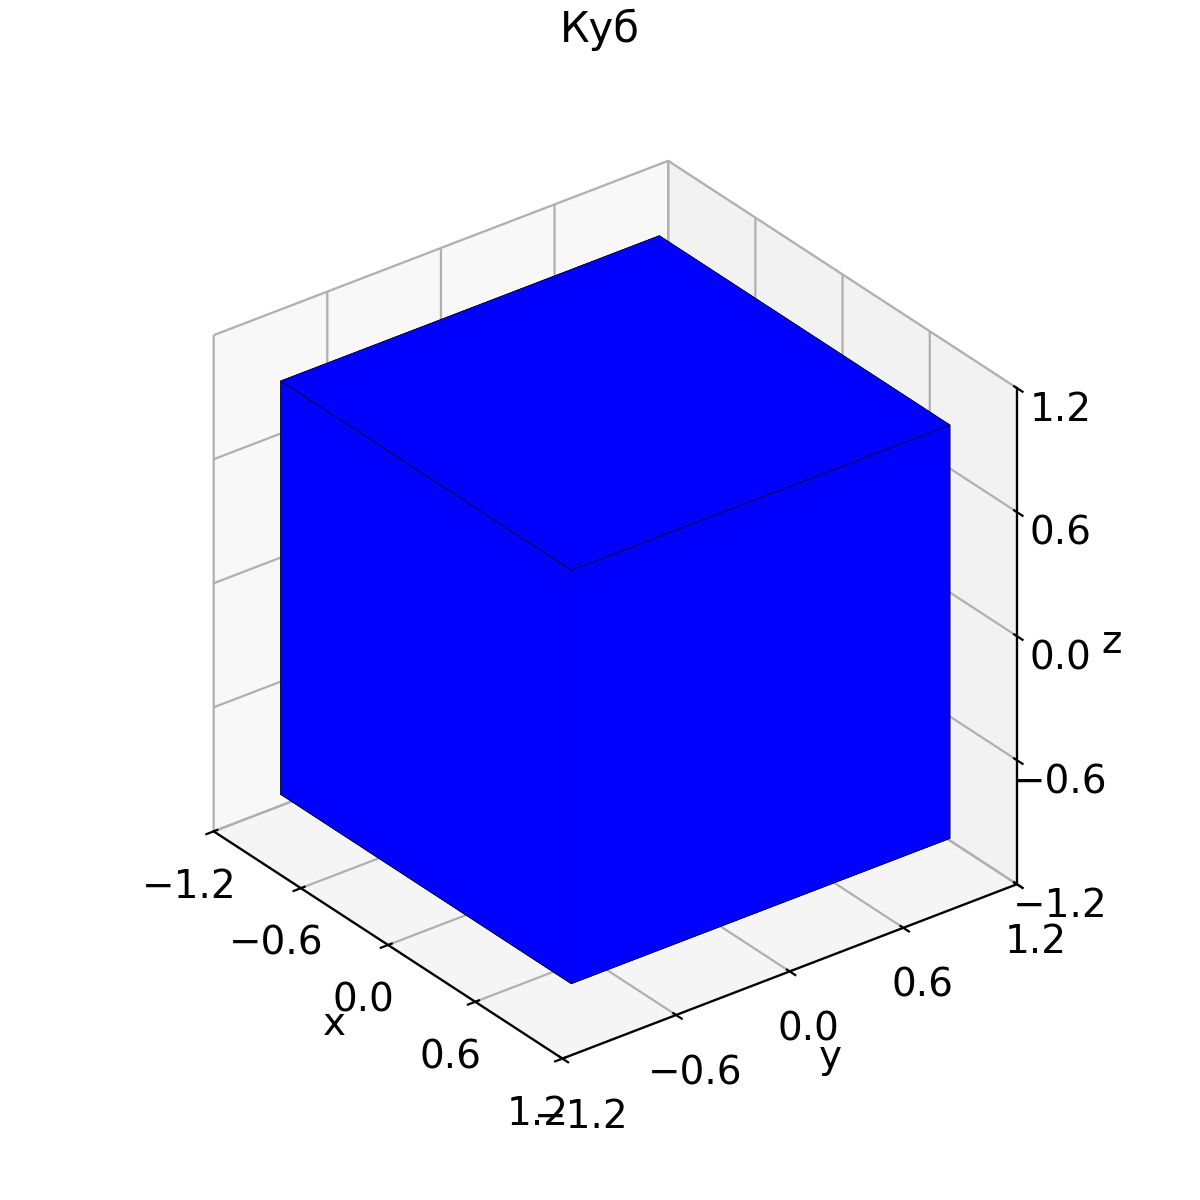
\includegraphics[width=0.49\linewidth]{figures/cube.png}
\hfill
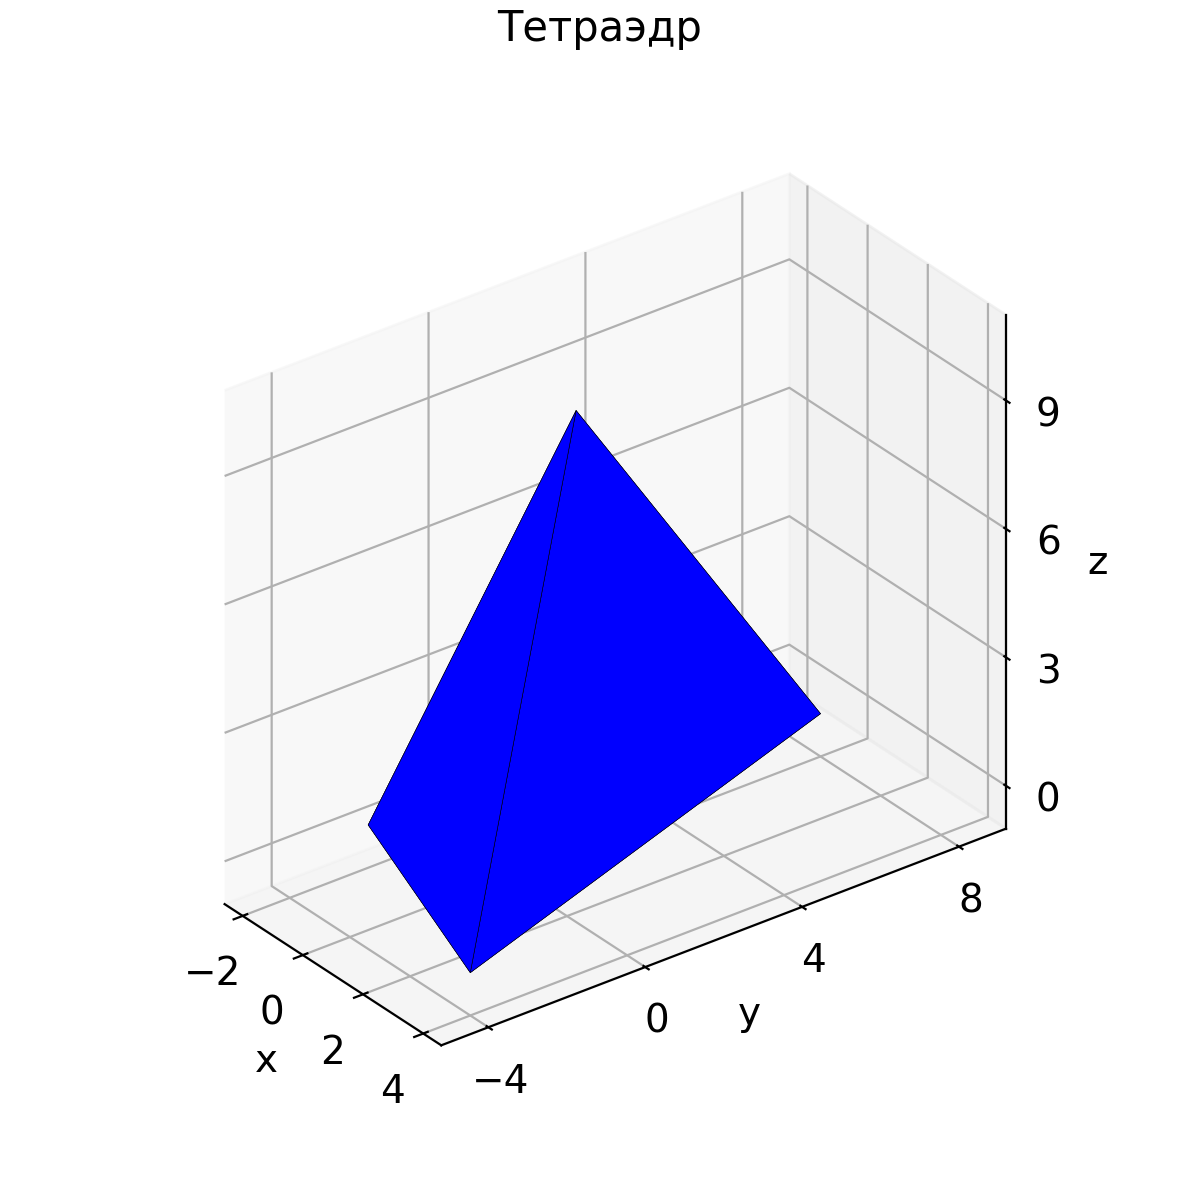
\includegraphics[width=0.49\linewidth]{figures/tetra.png}
\caption{Куб из методички и тетраэдр с выбранными вершинами}
\label{fig:p01_figures}
\end{figure}

\par\noindent\begin{minipage}{\linewidth}
\subsection*{Вывод по заданию 1}

Матрица $3\times3$ не может перенести начало
координат в другую точку, поскольку произведение любой матрицы на нулевой
вектор равно нулевому вектору. Четвёртая координата позволяет описать перенос
матричным умножением; перед отрисовкой однородные координаты переводятся
в декартовы делением на $w$.

\end{minipage}\par
\section{Задание 2. Масштабирование куба}

\subsection*{Общая структура матрицы}

Масштабирование по координатным осям задаётся матрицей

\begin{center}\adjustbox{max width=\linewidth}{$\displaystyle S(s_x,s_y,s_z)=\begin{pmatrix}
s_x&0&0&0\\
0&s_y&0&0\\
0&0&s_z&0\\
0&0&0&1
\end{pmatrix},\qquad
S\begin{pmatrix}x\\y\\z\\1\end{pmatrix}
=\begin{pmatrix}s_xx\\s_yy\\s_zz\\1\end{pmatrix}.$}\end{center}

Матрицы масштаба отдельно по $x$, $y$, $z$ получаются подстановкой
$(s_x,1,1)$, $(1,s_y,1)$, $(1,1,s_z)$ соответственно.
Все вершины преобразуются одновременно: $V'=SV$, в Python — \texttt{S @ vertices\_cube}.

\subsection*{Выбранные матрицы и их композиция}

\begin{center}\adjustbox{max width=\linewidth}{$\displaystyle S_1=\begin{pmatrix}
2&0&0&0\\
0&4&0&0\\
0&0&10&0\\
0&0&0&1
\end{pmatrix},\qquad
S_2=\begin{pmatrix}
0.5&0&0&0\\
0&1&0&0\\
0&0&0.1&0\\
0&0&0&1
\end{pmatrix}.$}\end{center}

Сначала применяется $S_1$, затем $S_2$. Для векторов-столбцов последняя
применяемая матрица стоит слева:

\begin{center}\adjustbox{max width=\linewidth}{$\displaystyle S_2(S_1V)=(S_2S_1)V,\qquad
S_2S_1=\operatorname{diag}(0.5\cdot2,\;1\cdot4,\;0.1\cdot10,\;1)
=\begin{pmatrix}
1&0&0&0\\
0&4&0&0\\
0&0&1&0\\
0&0&0&1
\end{pmatrix}.$}\end{center}

Отдельные матрицы $S_1$ и $S_2$ применяются к исходному кубу, а третий
результат соответствует их последовательному применению.

\begin{table}[H]\centering\singlespacing\small
\caption{Размеры куба после масштабирования}
\label{tab:scale_sizes}
\begin{adjustbox}{max width=\linewidth}
\begin{tabular}{llll}
\toprule
Преобразование & Размер по $x$ & Размер по $y$ & Размер по $z$ \\
\midrule
Исходный куб & 2 & 2 & 2 \\
$S_1$ & 4 & 8 & 20 \\
$S_2$ & 1 & 2 & 0.2 \\
$S_2S_1$ & 2 & 8 & 2 \\
\bottomrule\end{tabular}\end{adjustbox}\end{table}

Например, для вершины $p=(-1,-1,-1,1)^T$:

\begin{center}\adjustbox{max width=\linewidth}{$\displaystyle S_1p=(-2,-4,-10,1)^T,\quad
S_2p=(-0.5,-1,-0.1,1)^T,\quad
S_2S_1p=(-1,-4,-1,1)^T.$}\end{center}

Результаты приведены на рисунке~\ref{fig:p02_scaling}. У панелей разные пределы осей,
поэтому абсолютные размеры нужно сравнивать по численным отметкам и таблице.
Внутри каждой панели единичный масштаб одинаков по трём осям.

\begin{figure}[H]
\centering
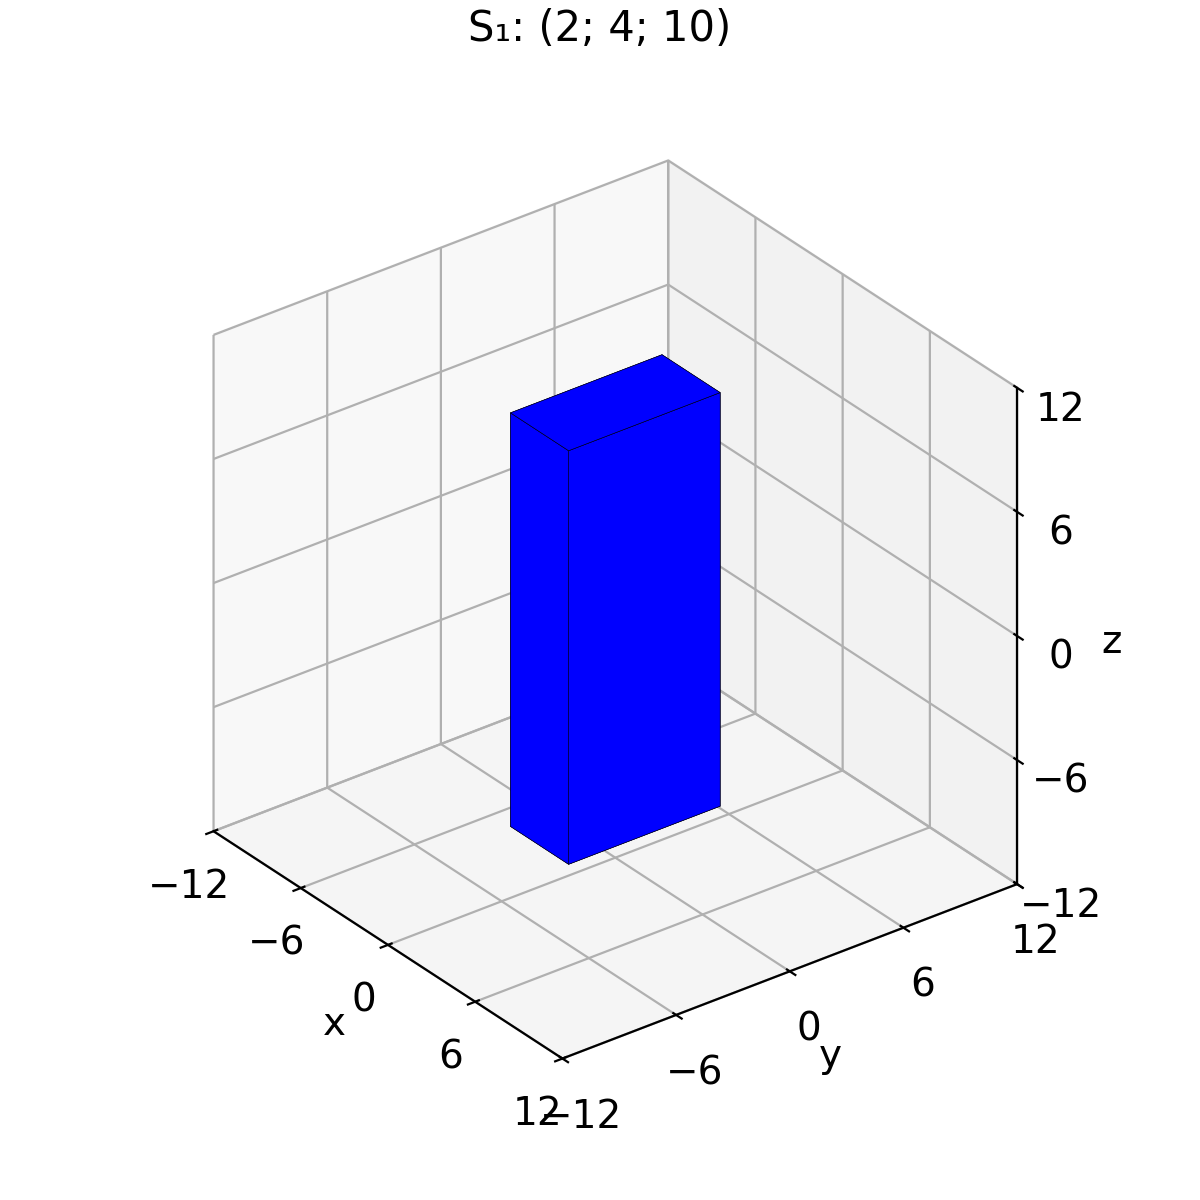
\includegraphics[width=0.49\linewidth]{figures/s1.png}
\hfill
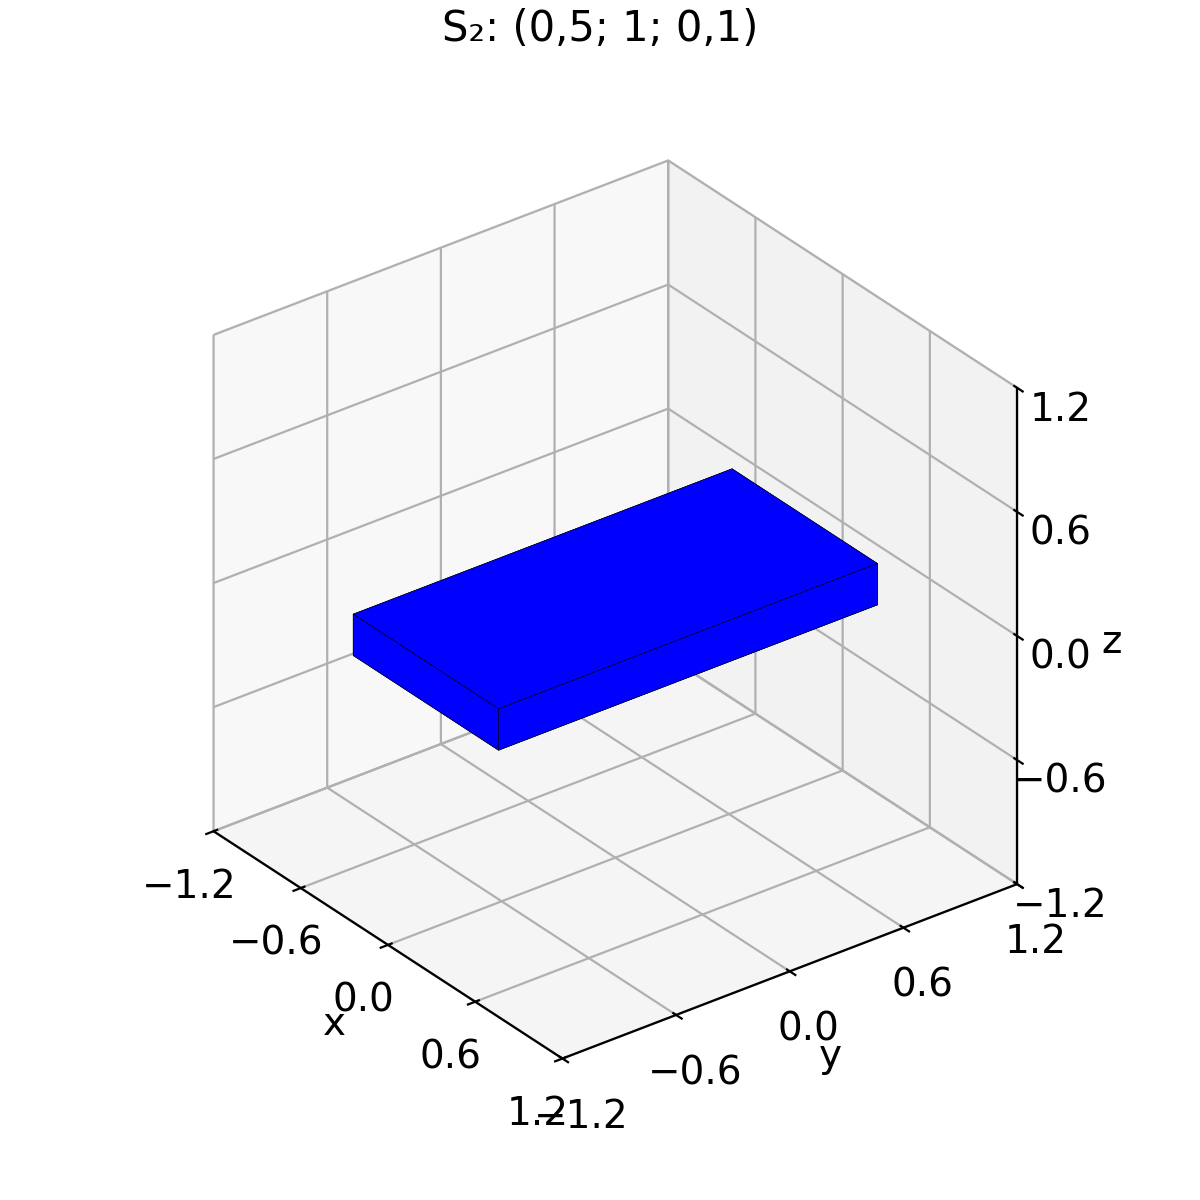
\includegraphics[width=0.49\linewidth]{figures/s2.png}
\par\medskip
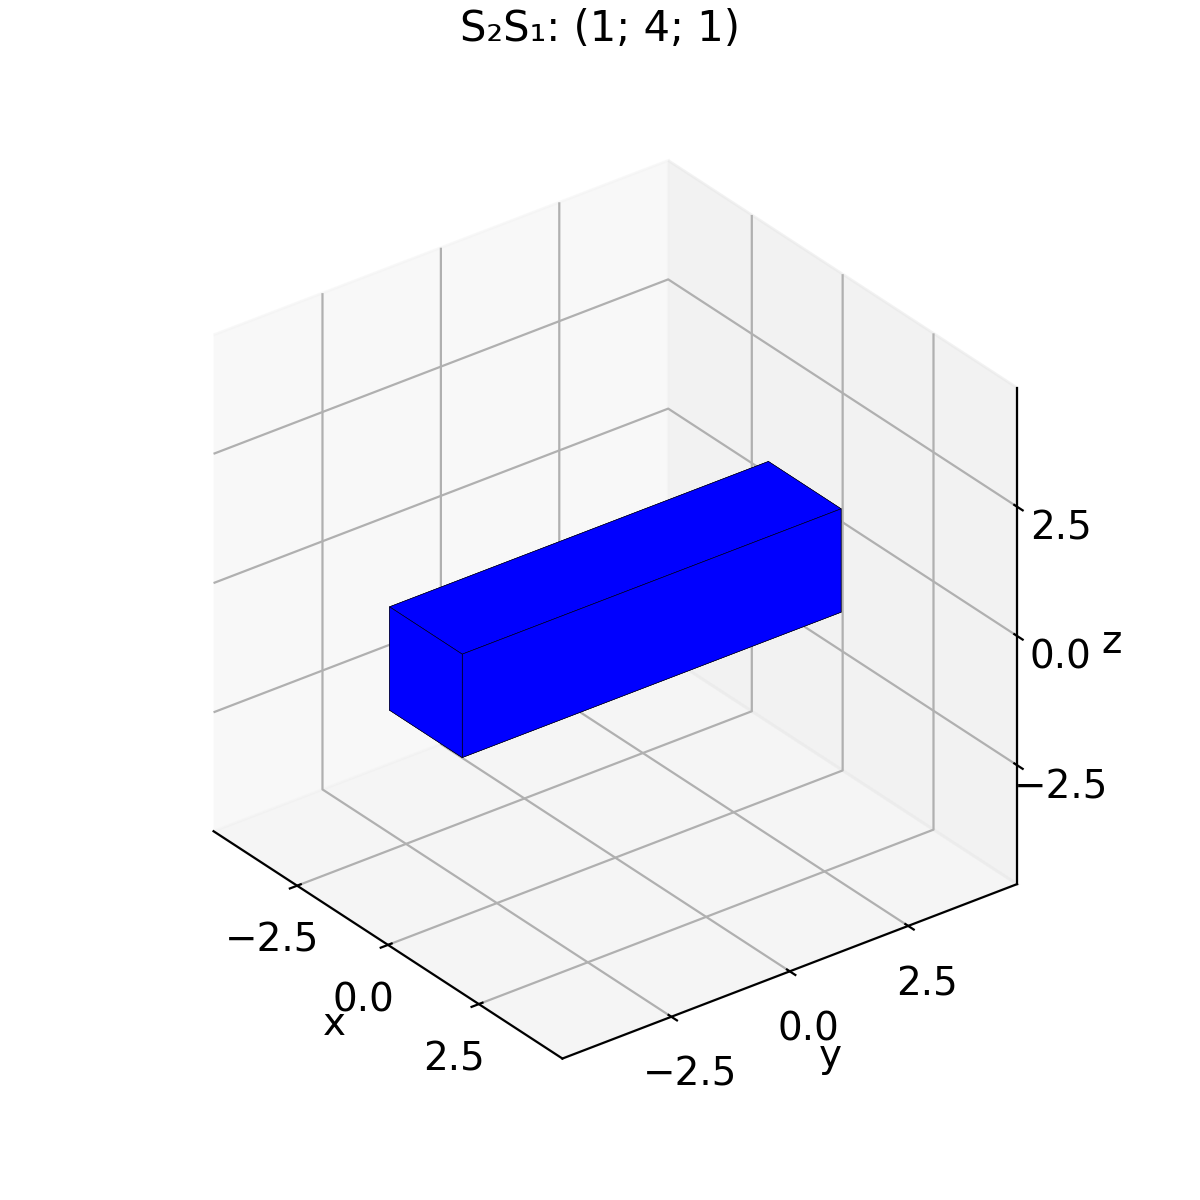
\includegraphics[width=0.49\linewidth]{figures/s21.png}
\caption{Два масштаба и их композиция}
\label{fig:p02_scaling}
\end{figure}

\par\noindent\begin{minipage}{\linewidth}
\subsection*{Вывод по заданию 2}

При последовательном масштабировании коэффициенты по каждой оси перемножаются.
По оси $x$ получаем $2\cdot0.5=1$, а по оси $z$ — $10\cdot0.1=1$:
второе преобразование компенсирует первое, поэтому размеры по этим осям
возвращаются к исходным. По оси $y$ произведение равно $4\cdot1=4$,
поэтому растяжение в четыре раза сохраняется. Результат композиции —
прямоугольный параллелепипед с размерами $(2,8,2)$.

\end{minipage}\par
\section{Задание 3. Перенос и порядок преобразований}

\subsection*{Общая структура матрицы переноса}

\begin{center}\adjustbox{max width=\linewidth}{$\displaystyle T(a,b,c)=\begin{pmatrix}
1&0&0&a\\
0&1&0&b\\
0&0&1&c\\
0&0&0&1
\end{pmatrix},\qquad
T\begin{pmatrix}x\\y\\z\\1\end{pmatrix}
=\begin{pmatrix}x+a\\y+b\\z+c\\1\end{pmatrix}.$}\end{center}

Переносы отдельно по $x$, $y$, $z$ задаются $T(a,0,0)$, $T(0,b,0)$,
$T(0,0,c)$ соответственно. Последний столбец добавляет смещение к координатам.

\subsection*{Выбранные переносы и композиция}

\begin{center}\adjustbox{max width=\linewidth}{$\displaystyle T_1=\begin{pmatrix}
1&0&0&5\\
0&1&0&5\\
0&0&1&2\\
0&0&0&1
\end{pmatrix},\qquad
T_2=\begin{pmatrix}
1&0&0&0\\
0&1&0&3\\
0&0&1&10\\
0&0&0&1
\end{pmatrix}.$}\end{center}

При последовательном применении векторы переноса складываются:

\begin{center}\adjustbox{max width=\linewidth}{$\displaystyle T_2T_1=T(5+0,\;5+3,\;2+10)
=\begin{pmatrix}
1&0&0&5\\
0&1&0&8\\
0&0&1&12\\
0&0&0&1
\end{pmatrix}.$}\end{center}

Центры образов куба равны $(5,5,2)$, $(0,3,10)$ и $(5,8,12)$ соответственно.
Для исходной вершины $p=(-1,-1,-1,1)^T$:

\begin{center}\adjustbox{max width=\linewidth}{$\displaystyle T_1p=(4,4,1,1)^T,\quad
T_2p=(-1,2,9,1)^T,\quad
T_2T_1p=(4,7,11,1)^T.$}\end{center}

Во всех трёх случаях размеры равны $(2,2,2)$. Результаты показаны на рисунке~\ref{fig:p03_translation}.
Серым пунктиром обозначен исходный куб; у трёх панелей одинаковые пределы осей.

\begin{figure}[H]
\centering
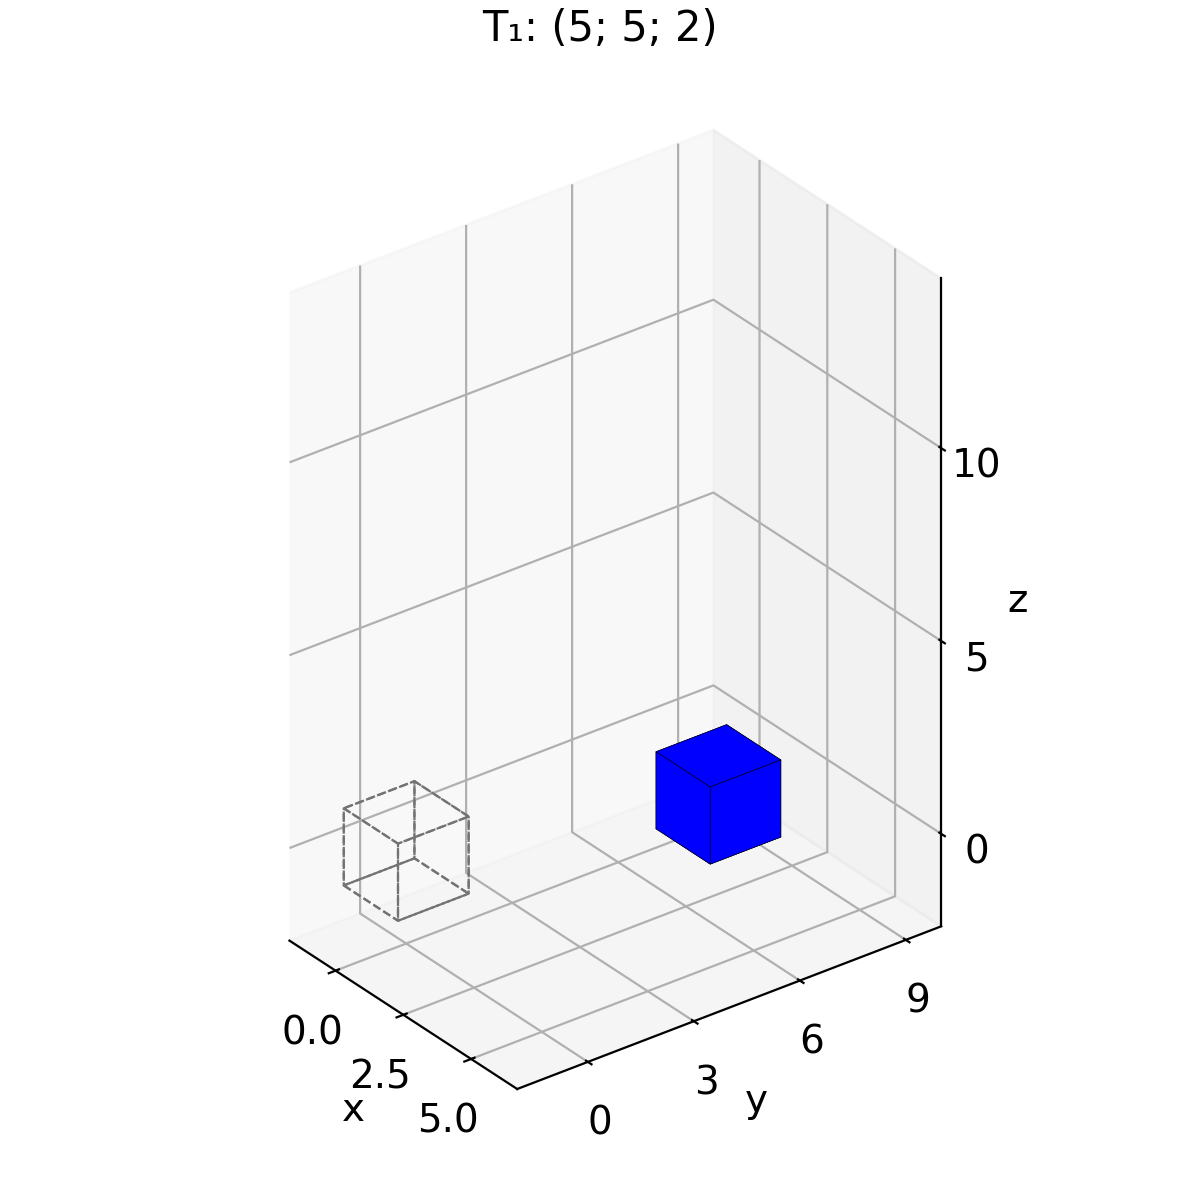
\includegraphics[width=0.49\linewidth]{figures/t1.png}
\hfill
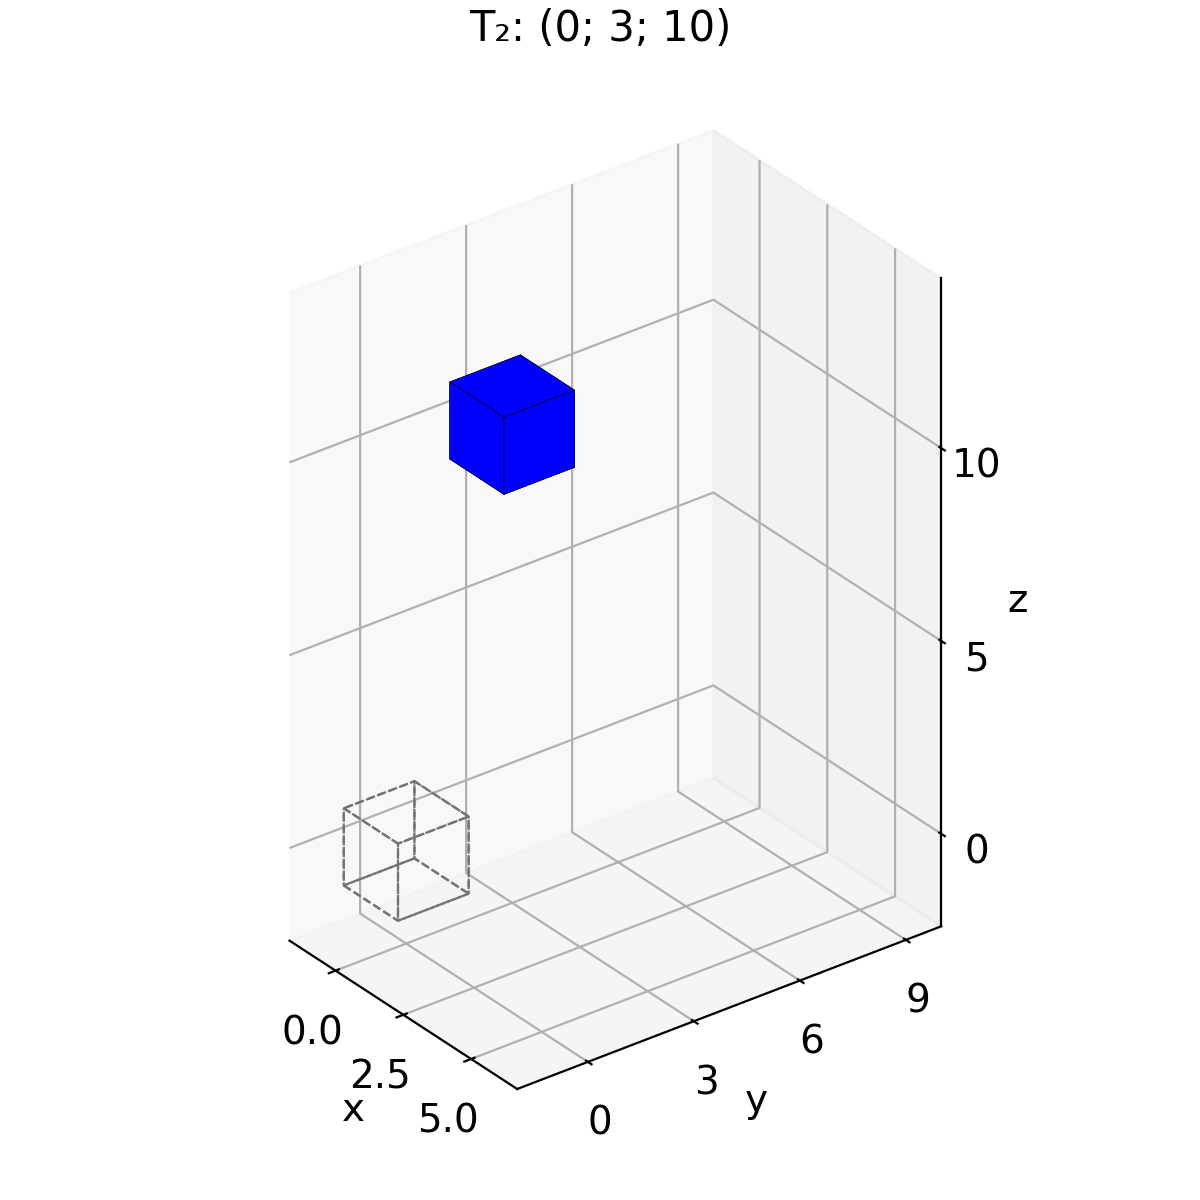
\includegraphics[width=0.49\linewidth]{figures/t2.png}
\par\medskip
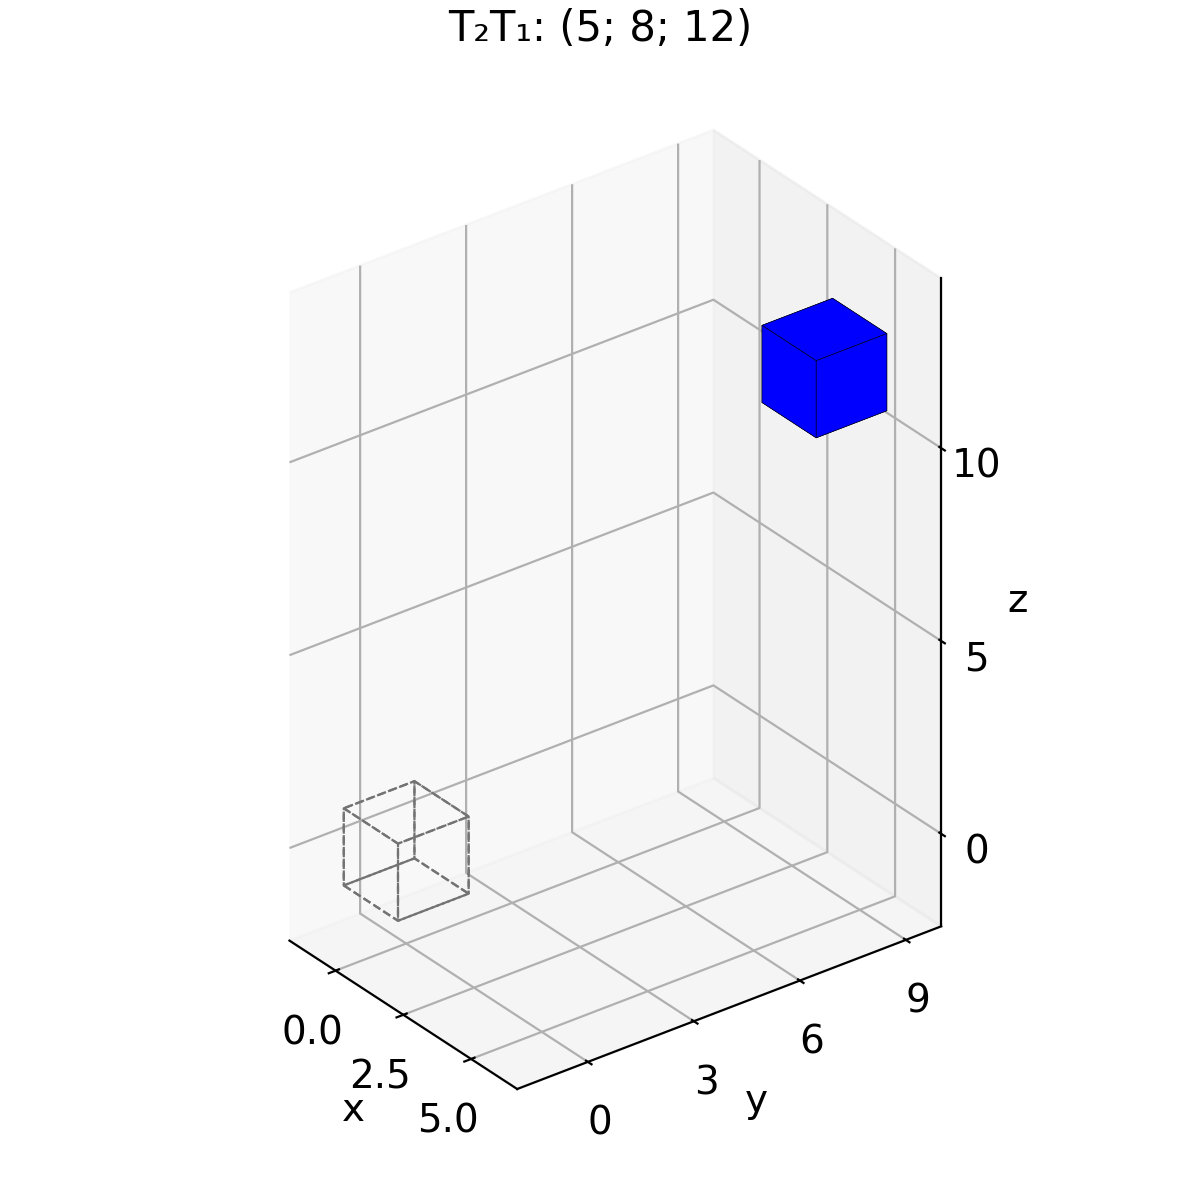
\includegraphics[width=0.49\linewidth]{figures/t21.png}
\caption{Два переноса и их композиция; исходный куб показан контуром}
\label{fig:p03_translation}
\end{figure}

\subsection*{Сравнение TS и ST}

Для сравнения выбраны $T=T_1$ и $S=S_1$:

\begin{center}\adjustbox{max width=\linewidth}{$\displaystyle TS=\begin{pmatrix}
2&0&0&5\\
0&4&0&5\\
0&0&10&2\\
0&0&0&1
\end{pmatrix},\qquad
ST=\begin{pmatrix}
2&0&0&10\\
0&4&0&20\\
0&0&10&20\\
0&0&0&1
\end{pmatrix}.$}\end{center}

При $TS$ точка сначала масштабируется, затем переносится:

\begin{center}\adjustbox{max width=\linewidth}{$\displaystyle (x,y,z)\longmapsto(2x+5,\;4y+5,\;10z+2).$}\end{center}

При $ST$ точка сначала переносится, затем масштабируется:

\begin{center}\adjustbox{max width=\linewidth}{$\displaystyle (x,y,z)\longmapsto(2(x+5),\;4(y+5),\;10(z+2))
=(2x+10,\;4y+20,\;10z+20).$}\end{center}

Например, $TSp=(3,1,-8,1)^T$, а $STp=(8,16,10,1)^T$.
Разность декартовых координат равна $(5,15,18)$ для каждой вершины.

\begin{table}[H]\centering\singlespacing\small
\caption{Центры и размеры образов TS и ST}
\label{tab:transform_order}
\begin{adjustbox}{max width=\linewidth}
\begin{tabular}{lll}
\toprule
Преобразование & Центр образа & Размеры по $x,y,z$ \\
\midrule
$TS$ & $(5,5,2)$ & $(4,8,20)$ \\
$ST$ & $(10,20,20)$ & $(4,8,20)$ \\
\bottomrule\end{tabular}\end{adjustbox}\end{table}

Результаты неэквивалентны: матрицы отличаются последним столбцом и дают
разные координаты образов. Сравнение приведено на рисунке~\ref{fig:p03_order}.

\begin{figure}[H]
\centering
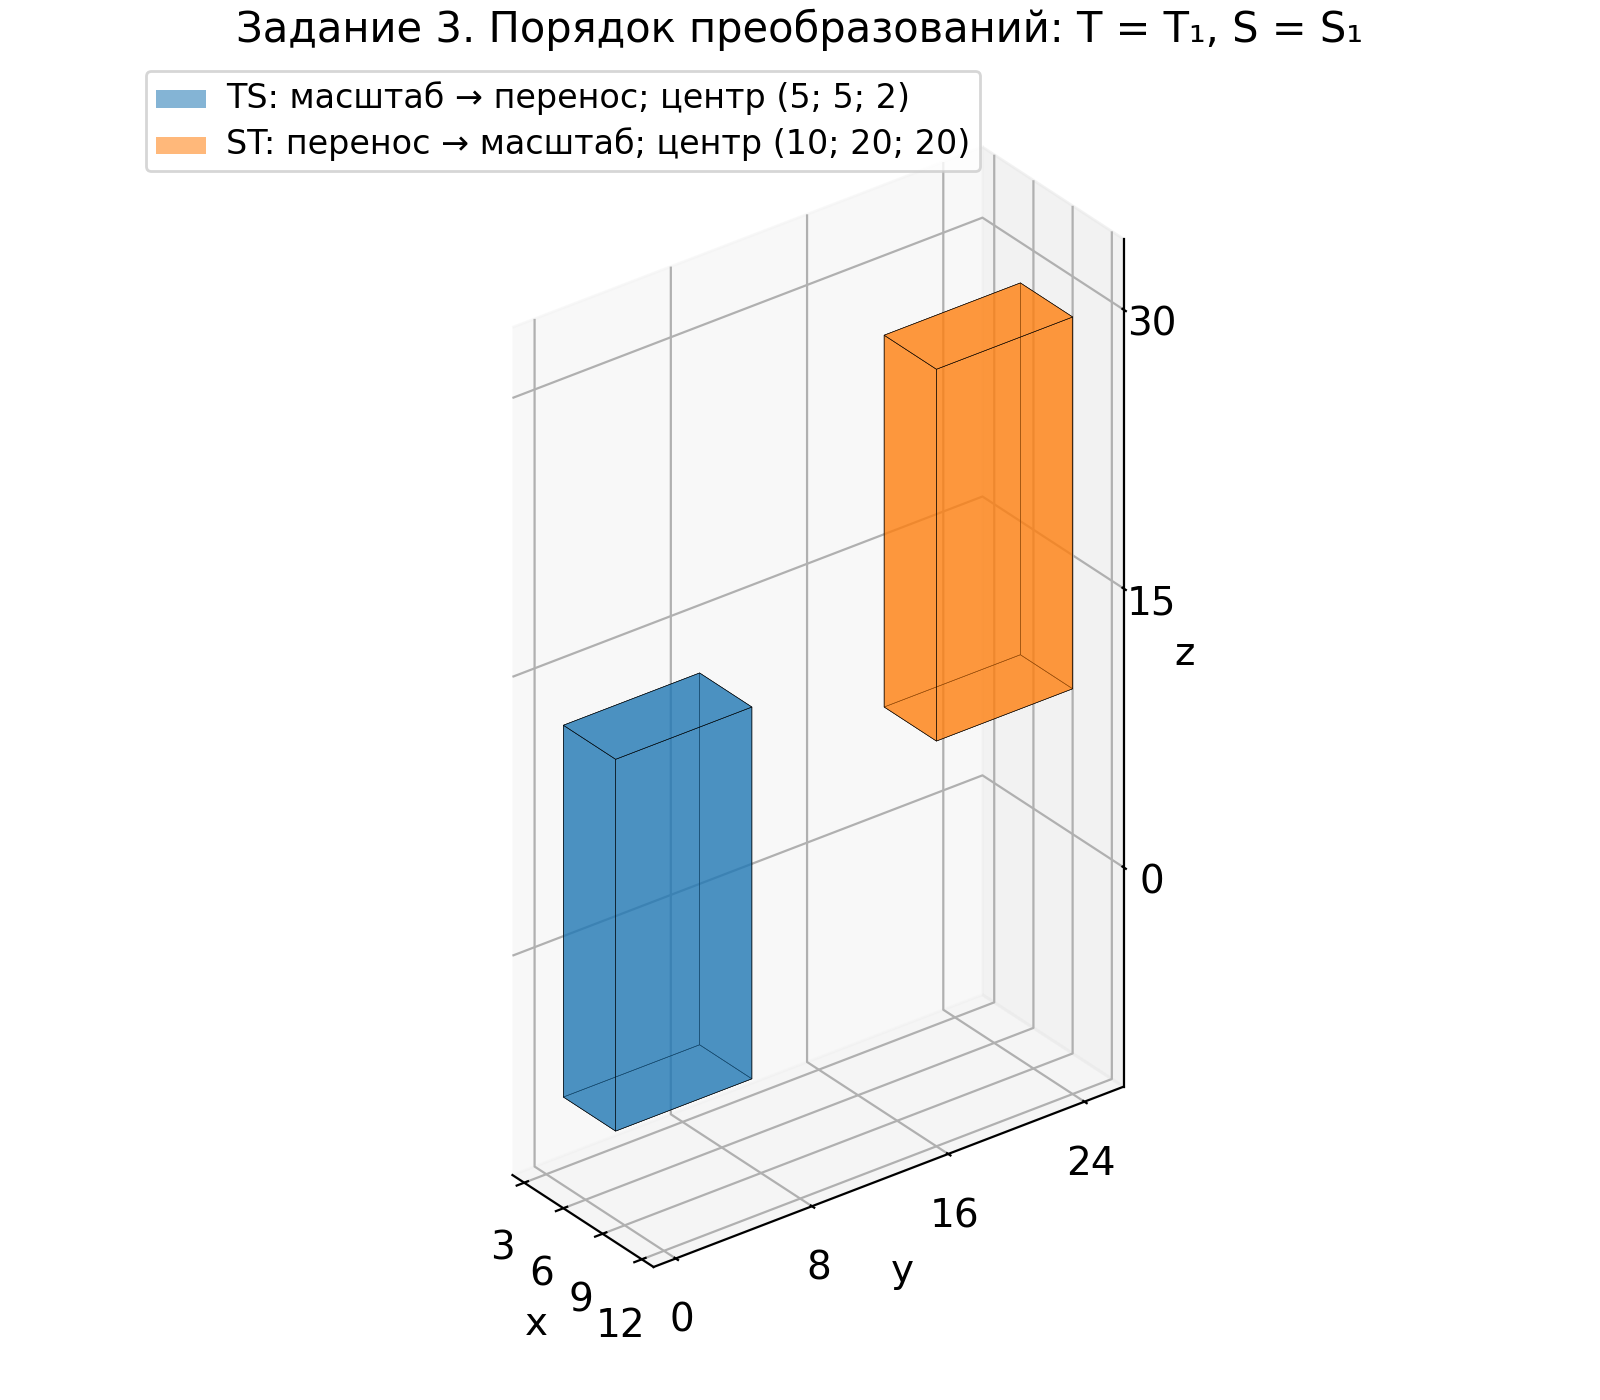
\includegraphics[width=0.83\linewidth]{figures/order.png}
\caption{Сравнение порядка применения масштабирования и переноса}
\label{fig:p03_order}
\end{figure}

\par\noindent\begin{minipage}{\linewidth}
\subsection*{Вывод по заданию 3}

Перенос добавляет один и тот же вектор ко всем вершинам, поэтому разности
их координат и размеры куба не меняются. Два последовательных переноса
равносильны одному переносу на сумму векторов: $(5,8,12)$.

В общем случае умножение матриц некоммутативно: порядок преобразований
может менять результат. Для выбранных матриц $TS\ne ST$. В $TS$ масштаб
применяется до переноса, а в $ST$ масштабируется и добавленное смещение:
$(5,5,2)$ превращается в $(2\cdot5,4\cdot5,10\cdot2)=(10,20,20)$.
Поэтому положения образов различаются. Размеры в обоих случаях одинаковы,
$(4,8,20)$, поскольку применяется один и тот же масштаб, а перенос размеры
не меняет.

Определители произведений совпадают:

\begin{center}\adjustbox{max width=\linewidth}{$\displaystyle \det(TS)=\det(T)\det(S)=\det(S)\det(T)=\det(ST)=1\cdot80=80.$}\end{center}

Это следует из коммутативности умножения чисел и означает одинаковое
изменение объёма — в $80$ раз. Само по себе равенство определителей
не гарантирует одинаковых размеров или положения фигур.
\end{minipage}\par
\clearpage
\section{Задание 4. Вращение кубика}

\subsection*{Постановка задачи}

Требуется повернуть кубик вокруг произвольной оси, проходящей через его центр. Ось вращения задается вектором

\begin{center}\adjustbox{max width=\linewidth}{$\displaystyle v =
\begin{bmatrix}
v_x \\
v_y \\
v_z
\end{bmatrix},$}\end{center}

а угол поворота — величиной $\theta$. Матрица поворота определяется через матричную экспоненту:

\begin{center}\adjustbox{max width=\linewidth}{$\displaystyle R_v(\theta) = e^{J\theta},
\qquad
J =
\frac{1}{\|v\|}
\begin{bmatrix}
0 & -v_z & v_y & 0 \\
v_z & 0 & -v_x & 0 \\
-v_y & v_x & 0 & 0 \\
0 & 0 & 0 & 0
\end{bmatrix}.$}\end{center}

Матрица $J$ имеет размер $4 \times 4$, поскольку вершины кубика заданы в однородных координатах. Последняя строка и последний столбец матрицы $J$ нулевые, поэтому в матричной экспоненте в правом нижнем углу стоит единица, а четвертая координата остается равной единице. Следовательно, преобразование является аффинным.

\subsection*{Исходные данные}

Кубик задан в однородных координатах. Его вершины являются столбцами матрицы

\begin{center}\adjustbox{max width=\linewidth}{$\displaystyle V =
\begin{bmatrix}
-1 & 1 & 1 & -1 & -1 & 1 & 1 & -1 \\
-1 & -1 & 1 & 1 & -1 & -1 & 1 & 1 \\
-1 & -1 & -1 & -1 & 1 & 1 & 1 & 1 \\
1 & 1 & 1 & 1 & 1 & 1 & 1 & 1
\end{bmatrix}.$}\end{center}

Центр кубика совпадает с началом координат, поэтому ось вращения, проходящая через центр кубика, проходит через точку $(0,0,0)$, и отдельная матрица переноса не требуется.

\subsection*{Общая структура матрицы поворота}

Пусть

\begin{center}\adjustbox{max width=\linewidth}{$\displaystyle u =
\frac{v}{\|v\|}
=
\begin{bmatrix}
u_x \\
u_y \\
u_z
\end{bmatrix},
\qquad
\|u\| = 1$}\end{center}

— нормированный вектор оси вращения. Кососимметрическая матрица, соответствующая этому вектору, имеет вид

\begin{center}\adjustbox{max width=\linewidth}{$\displaystyle K =
\begin{bmatrix}
0 & -u_z & u_y & 0 \\
u_z & 0 & -u_x & 0 \\
-u_y & u_x & 0 & 0 \\
0 & 0 & 0 & 0
\end{bmatrix}.$}\end{center}

Для нормированного вектора $u$ выполняется свойство

\begin{center}\adjustbox{max width=\linewidth}{$\displaystyle K^3 = -K.$}\end{center}

Поэтому матричная экспонента приводится к формуле Родригеса:

\begin{center}\adjustbox{max width=\linewidth}{$\displaystyle R_u(\theta) = e^{K\theta}
=
I + \sin\theta \, K + (1-\cos\theta)K^2.$}\end{center}

Для компактной записи положим $c=\cos\theta$, $s=\sin\theta$, $d=1-c$. Матрица поворота вокруг произвольной оси, проходящей через начало координат, имеет вид

\begin{center}\adjustbox{max width=\linewidth}{$\displaystyle R_u(\theta) =
\begin{bmatrix}
c+u_x^2d & u_xu_yd-u_zs & u_xu_zd+u_ys & 0 \\
u_yu_xd+u_zs & c+u_y^2d & u_yu_zd-u_xs & 0 \\
u_zu_xd-u_ys & u_zu_yd+u_xs & c+u_z^2d & 0 \\
0 & 0 & 0 & 1
\end{bmatrix}.$}\end{center}

В программе матрица вычисляется напрямую по формуле $R_v(\theta)=e^{J\theta}$ с помощью \texttt{scipy.linalg.expm}; формула Родригеса приведена выше для аналитической записи этой же матрицы.

\subsection*{Матрицы поворота вокруг координатных осей}

Частными случаями общей формулы являются повороты вокруг осей $x$, $y$ и $z$.

Поворот вокруг оси $x$:

\begin{center}\adjustbox{max width=\linewidth}{$\displaystyle R_x(\theta) =
\begin{bmatrix}
1 & 0 & 0 & 0 \\
0 & \cos\theta & -\sin\theta & 0 \\
0 & \sin\theta & \cos\theta & 0 \\
0 & 0 & 0 & 1
\end{bmatrix}.$}\end{center}

Поворот вокруг оси $y$:

\begin{center}\adjustbox{max width=\linewidth}{$\displaystyle R_y(\theta) =
\begin{bmatrix}
\cos\theta & 0 & \sin\theta & 0 \\
0 & 1 & 0 & 0 \\
-\sin\theta & 0 & \cos\theta & 0 \\
0 & 0 & 0 & 1
\end{bmatrix}.$}\end{center}

Поворот вокруг оси $z$:

\begin{center}\adjustbox{max width=\linewidth}{$\displaystyle R_z(\theta) =
\begin{bmatrix}
\cos\theta & -\sin\theta & 0 & 0 \\
\sin\theta & \cos\theta & 0 & 0 \\
0 & 0 & 1 & 0 \\
0 & 0 & 0 & 1
\end{bmatrix}.$}\end{center}

Эти матрицы получаются из общей формулы при выборе единичных векторов

\begin{center}\adjustbox{max width=\linewidth}{$\displaystyle e_x =
\begin{bmatrix}
1 \\
0 \\
0
\end{bmatrix},
\qquad
e_y =
\begin{bmatrix}
0 \\
1 \\
0
\end{bmatrix},
\qquad
e_z =
\begin{bmatrix}
0 \\
0 \\
1
\end{bmatrix}.$}\end{center}

\subsection*{Выбранные оси и углы поворота}

Для выполнения задания выбраны две произвольные оси вращения и два угла поворота.

Первая ось:

\begin{center}\adjustbox{max width=\linewidth}{$\displaystyle v_1 =
\begin{bmatrix}
1 \\
1 \\
0
\end{bmatrix},
\qquad
\theta_1 = \frac{\pi}{2},
\qquad
u_1 =
\frac{v_1}{\|v_1\|}
=
\begin{bmatrix}
\frac{1}{\sqrt{2}} \\
\frac{1}{\sqrt{2}} \\
0
\end{bmatrix}.$}\end{center}

Ось $v_1$ проходит через центр кубика и направлена вдоль диагонали плоскости $xy$.

Вторая ось:

\begin{center}\adjustbox{max width=\linewidth}{$\displaystyle v_2 =
\begin{bmatrix}
0 \\
1 \\
1
\end{bmatrix},
\qquad
\theta_2 = \frac{\pi}{3},
\qquad
u_2 =
\frac{v_2}{\|v_2\|}
=
\begin{bmatrix}
0 \\
\frac{1}{\sqrt{2}} \\
\frac{1}{\sqrt{2}}
\end{bmatrix}.$}\end{center}

Ось $v_2$ проходит через центр кубика и направлена вдоль диагонали плоскости $yz$.

\subsection*{Матрица первого поворота}

Для оси $v_1$ и угла $\theta_1=\frac{\pi}{2}$ имеем

\begin{center}\adjustbox{max width=\linewidth}{$\displaystyle \sin\frac{\pi}{2} = 1,
\qquad
\cos\frac{\pi}{2} = 0.$}\end{center}

Подстановка в общую формулу дает

\begin{center}\adjustbox{max width=\linewidth}{$\displaystyle \begin{gathered}
R_1 =
\begin{bmatrix}
\frac{1}{2} & \frac{1}{2} & \frac{1}{\sqrt{2}} & 0 \\
\frac{1}{2} & \frac{1}{2} & -\frac{1}{\sqrt{2}} & 0 \\
-\frac{1}{\sqrt{2}} & \frac{1}{\sqrt{2}} & 0 & 0 \\
0 & 0 & 0 & 1
\end{bmatrix} \\[4pt]
\approx \begin{bmatrix}
0.500000 & 0.500000 & 0.707107 & 0 \\
0.500000 & 0.500000 & -0.707107 & 0 \\
-0.707107 & 0.707107 & 0.000000 & 0 \\
0 & 0 & 0 & 1
\end{bmatrix}.
\end{gathered}$}\end{center}

Эта матрица выполняет поворот кубика на $90^\circ$ вокруг оси, направленной вдоль вектора $v_1$.

Проверим, что точка на оси вращения остается неподвижной. Возьмем точку

\begin{center}\adjustbox{max width=\linewidth}{$\displaystyle p =
\begin{bmatrix}
1 \\
1 \\
0 \\
1
\end{bmatrix}.$}\end{center}

Тогда

\begin{center}\adjustbox{max width=\linewidth}{$\displaystyle R_1 p =
\begin{bmatrix}
1 \\
1 \\
0 \\
1
\end{bmatrix}
= p.$}\end{center}

Следовательно, прямая, проходящая через начало координат вдоль вектора $v_1$, действительно является осью вращения.

\subsection*{Матрица второго поворота}

Для оси $v_2$ и угла $\theta_2=\frac{\pi}{3}$ имеем

\begin{center}\adjustbox{max width=\linewidth}{$\displaystyle \sin\frac{\pi}{3} = \frac{\sqrt{3}}{2},
\qquad
\cos\frac{\pi}{3} = \frac{1}{2}.$}\end{center}

После подстановки в общую формулу получаем

\begin{center}\adjustbox{max width=\linewidth}{$\displaystyle \begin{gathered}
R_2 =
\begin{bmatrix}
\frac{1}{2} & -\frac{\sqrt{6}}{4} & \frac{\sqrt{6}}{4} & 0 \\
\frac{\sqrt{6}}{4} & \frac{3}{4} & \frac{1}{4} & 0 \\
-\frac{\sqrt{6}}{4} & \frac{1}{4} & \frac{3}{4} & 0 \\
0 & 0 & 0 & 1
\end{bmatrix} \\[4pt]
\approx \begin{bmatrix}
0.500000 & -0.612372 & 0.612372 & 0 \\
0.612372 & 0.750000 & 0.250000 & 0 \\
-0.612372 & 0.250000 & 0.750000 & 0 \\
0 & 0 & 0 & 1
\end{bmatrix}.
\end{gathered}$}\end{center}

Эта матрица выполняет поворот кубика на $60^\circ$ вокруг оси, направленной вдоль вектора $v_2$.

Проверка неподвижности оси:

\begin{center}\adjustbox{max width=\linewidth}{$\displaystyle p =
\begin{bmatrix}
0 \\
1 \\
1 \\
1
\end{bmatrix},
\qquad
R_2 p =
\begin{bmatrix}
0 \\
1 \\
1 \\
1
\end{bmatrix}
= p.$}\end{center}

Следовательно, ось вращения задана корректно.

\subsection*{Композиция двух поворотов}

Поскольку вершины кубика рассматриваются как столбцы матрицы $V$, преобразование применяется умножением матрицы слева:

\begin{center}\adjustbox{max width=\linewidth}{$\displaystyle V' = R V.$}\end{center}

Если сначала выполняется поворот $R_1$, а затем $R_2$, итоговая матрица имеет вид

\begin{center}\adjustbox{max width=\linewidth}{$\displaystyle M_{1 \to 2} = R_2 R_1.$}\end{center}

Если сначала выполняется поворот $R_2$, а затем $R_1$, итоговая матрица имеет вид

\begin{center}\adjustbox{max width=\linewidth}{$\displaystyle M_{2 \to 1} = R_1 R_2.$}\end{center}

В общем случае повороты в трехмерном пространстве не коммутируют, поэтому $R_2R_1 \neq R_1R_2$.

\subsection*{Композиция $M_{1 \to 2} = R_2R_1$}

Сначала выполняется поворот вокруг оси $v_1$ на угол $\theta_1=\frac{\pi}{2}$, затем — поворот вокруг оси $v_2$ на угол $\theta_2=\frac{\pi}{3}$. Численно:

\begin{center}\adjustbox{max width=\linewidth}{$\displaystyle M_{1 \to 2} \approx
\begin{bmatrix}
-0.489199 & 0.376826 & 0.786566 & 0 \\
0.504410 & 0.857963 & -0.097317 & 0 \\
-0.711516 & 0.349144 & -0.609789 & 0 \\
0 & 0 & 0 & 1
\end{bmatrix}.$}\end{center}

Результирующее преобразование также является поворотом вокруг некоторой оси. Нормированный вектор эквивалентной оси вращения приближенно равен

\begin{center}\adjustbox{max width=\linewidth}{$\displaystyle u_{1 \to 2} \approx
\begin{bmatrix}
0.2847 \\
0.9552 \\
0.0813
\end{bmatrix}.$}\end{center}

\subsection*{Композиция $M_{2 \to 1} = R_1R_2$}

Сначала выполняется поворот вокруг оси $v_2$ на угол $\theta_2=\frac{\pi}{3}$, затем — поворот вокруг оси $v_1$ на угол $\theta_1=\frac{\pi}{2}$. Численно:

\begin{center}\adjustbox{max width=\linewidth}{$\displaystyle M_{2 \to 1} \approx
\begin{bmatrix}
0.123174 & 0.245590 & 0.961516 & 0 \\
0.989199 & -0.107963 & -0.099144 & 0 \\
0.079459 & 0.963343 & -0.256236 & 0 \\
0 & 0 & 0 & 1
\end{bmatrix}.$}\end{center}

Нормированный вектор эквивалентной оси вращения приближенно равен

\begin{center}\adjustbox{max width=\linewidth}{$\displaystyle u_{2 \to 1} \approx
\begin{bmatrix}
0.6774 \\
0.5624 \\
0.4741
\end{bmatrix}.$}\end{center}

\subsection*{Демонстрация некоммутативности поворотов}

Сравним полученные матрицы:

\begin{center}\adjustbox{max width=\linewidth}{$\displaystyle M_{1 \to 2} = R_2R_1,
\qquad
M_{2 \to 1} = R_1R_2.$}\end{center}

Видно, что $M_{1 \to 2} \neq M_{2 \to 1}$. Например, элемент в первой строке и первом столбце:

\begin{center}\adjustbox{max width=\linewidth}{$\displaystyle (M_{1 \to 2})_{11} \approx -0.489199,
\qquad
(M_{2 \to 1})_{11} \approx 0.123174.$}\end{center}

Следовательно, порядок применения поворотов существенно влияет на итоговое положение кубика: последовательные повороты вокруг различных осей в трехмерном пространстве не коммутируют.

\subsection*{Результаты выполнения программы}

На каждом графике показаны исходный кубик (синий, полупрозрачный), кубик после применения соответствующей матрицы (красный), пунктирная ось вращения и вектор, коллинеарный этой оси. Для композиций на графиках показана эквивалентная ось результирующего поворота.

После применения любой из матриц четвертая однородная координата остается равной единице, поэтому в таблицах приведены только декартовы координаты $x$, $y$ и $z$.

\clearpage
\subsection*{Поворот вокруг оси $v_1$}

Применяется матрица $R_1$. Ось вращения — $v_1=(1,1,0)^T$, угол поворота — $\theta_1=\frac{\pi}{2}$. Ожидаемый результат: кубик повернут на $90^\circ$ вокруг диагонали плоскости $xy$.

Результат показан на рисунке~\ref{fig:p4A}, координаты вершин приведены в таблице~\ref{tab:p4A}.

\begin{figure}[H]
\centering
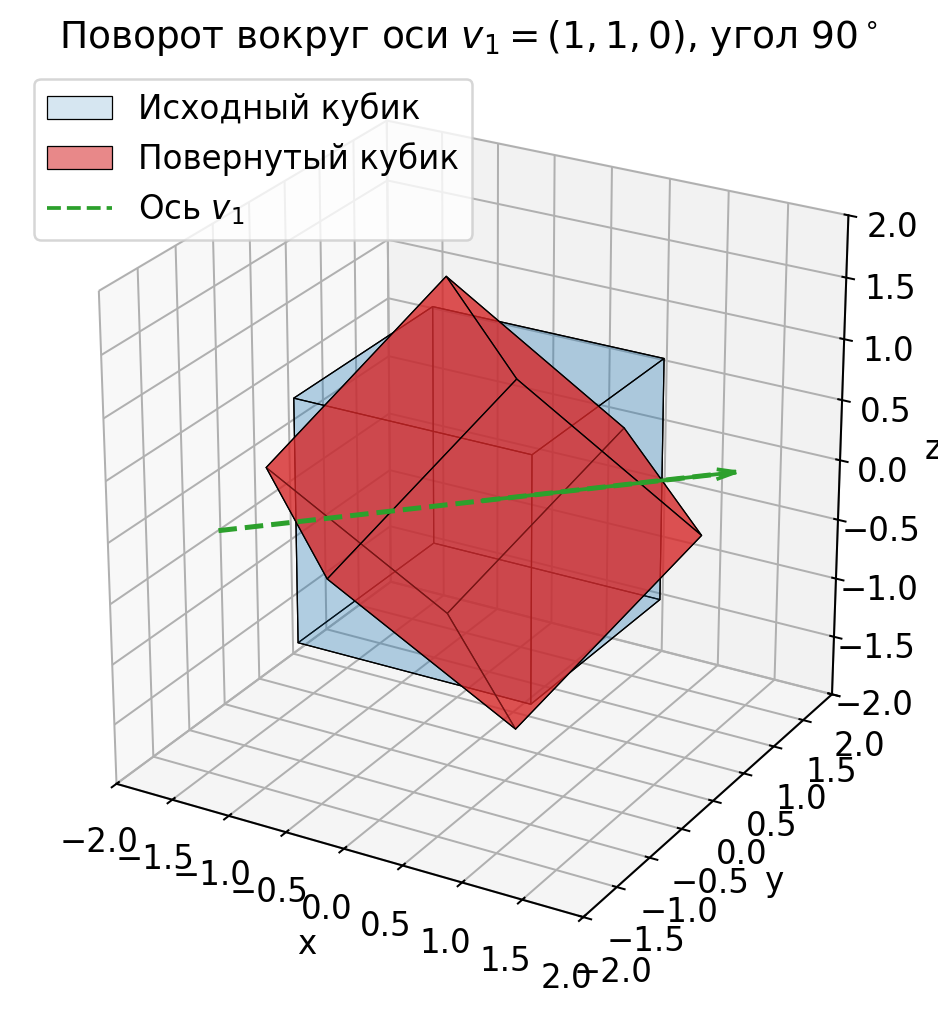
\includegraphics[width=0.66\linewidth]{figures/p4A.png}
\caption{Поворот на $90^\circ$ вокруг оси $v_1=(1,1,0)$}
\label{fig:p4A}
\end{figure}


\begin{table}[H]\centering\singlespacing\small
\caption{Координаты вершин после применения $R_1$}
\label{tab:p4A}
\begin{adjustbox}{max width=\linewidth}
\begin{tabular}{llll}
\toprule
№ вершины & $x$ & $y$ & $z$ \\
\midrule
1 & -1.707 & -0.293 & 0.000 \\
2 & -0.707 & 0.707 & -1.414 \\
3 & 0.293 & 1.707 & 0.000 \\
4 & -0.707 & 0.707 & 1.414 \\
5 & -0.293 & -1.707 & 0.000 \\
6 & 0.707 & -0.707 & -1.414 \\
7 & 1.707 & 0.293 & 0.000 \\
8 & 0.707 & -0.707 & 1.414 \\
\bottomrule\end{tabular}\end{adjustbox}\end{table}

\clearpage
\subsection*{Поворот вокруг оси $v_2$}

Применяется матрица $R_2$. Ось вращения — $v_2=(0,1,1)^T$, угол поворота — $\theta_2=\frac{\pi}{3}$. Ожидаемый результат: кубик повернут на $60^\circ$ вокруг диагонали плоскости $yz$.

Результат показан на рисунке~\ref{fig:p4B}, координаты вершин приведены в таблице~\ref{tab:p4B}.

\begin{figure}[H]
\centering
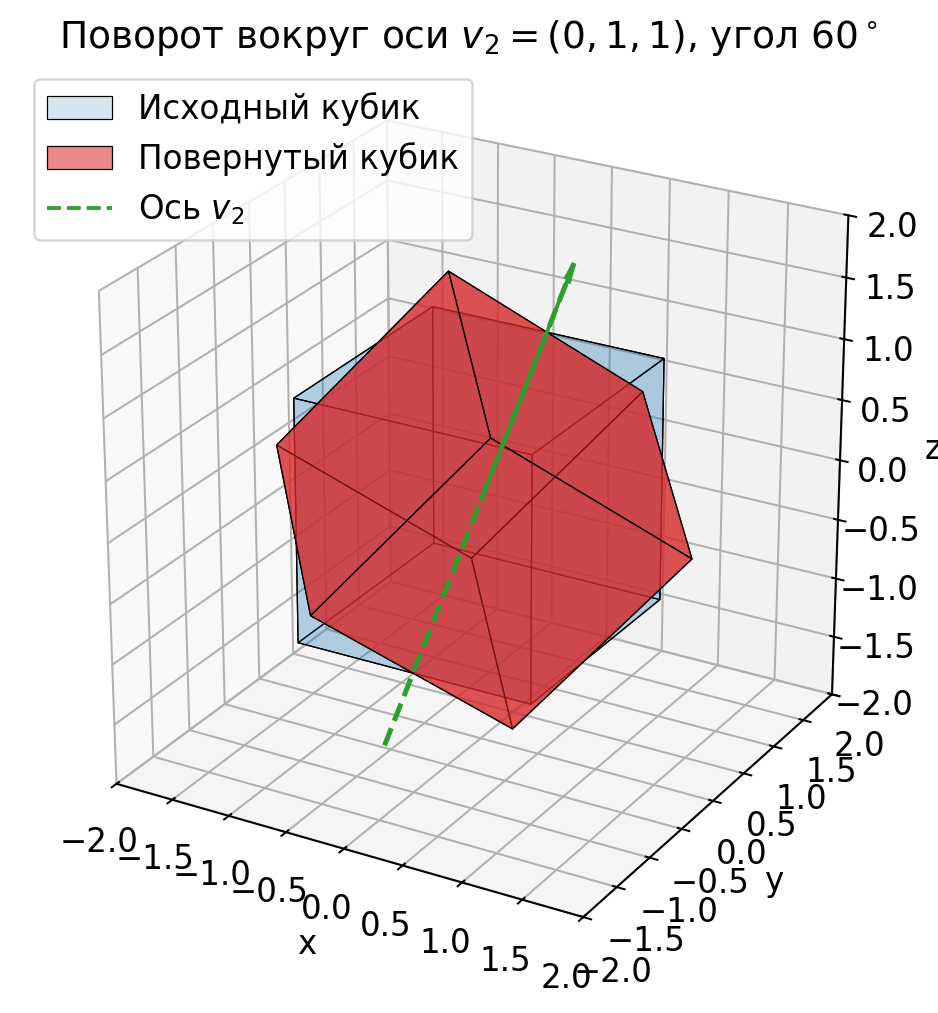
\includegraphics[width=0.66\linewidth]{figures/p4B.png}
\caption{Поворот на $60^\circ$ вокруг оси $v_2=(0,1,1)$}
\label{fig:p4B}
\end{figure}


\begin{table}[H]\centering\singlespacing\small
\caption{Координаты вершин после применения $R_2$}
\label{tab:p4B}
\begin{adjustbox}{max width=\linewidth}
\begin{tabular}{llll}
\toprule
№ вершины & $x$ & $y$ & $z$ \\
\midrule
1 & -0.500 & -1.612 & -0.388 \\
2 & 0.500 & -0.388 & -1.612 \\
3 & -0.725 & 1.112 & -1.112 \\
4 & -1.725 & -0.112 & 0.112 \\
5 & 0.725 & -1.112 & 1.112 \\
6 & 1.725 & 0.112 & -0.112 \\
7 & 0.500 & 1.612 & 0.388 \\
8 & -0.500 & 0.388 & 1.612 \\
\bottomrule\end{tabular}\end{adjustbox}\end{table}

\clearpage
\subsection*{Композиция $M_{1 \to 2}=R_2R_1$}

Порядок преобразований: сначала поворот вокруг оси $v_1$, затем поворот вокруг оси $v_2$. Эквивалентная ось вращения — $u_{1 \to 2}\approx(0.2847,\;0.9552,\;0.0813)^T$.

Результат показан на рисунке~\ref{fig:p4AB}, координаты вершин приведены в таблице~\ref{tab:p4AB}.

\begin{figure}[H]
\centering
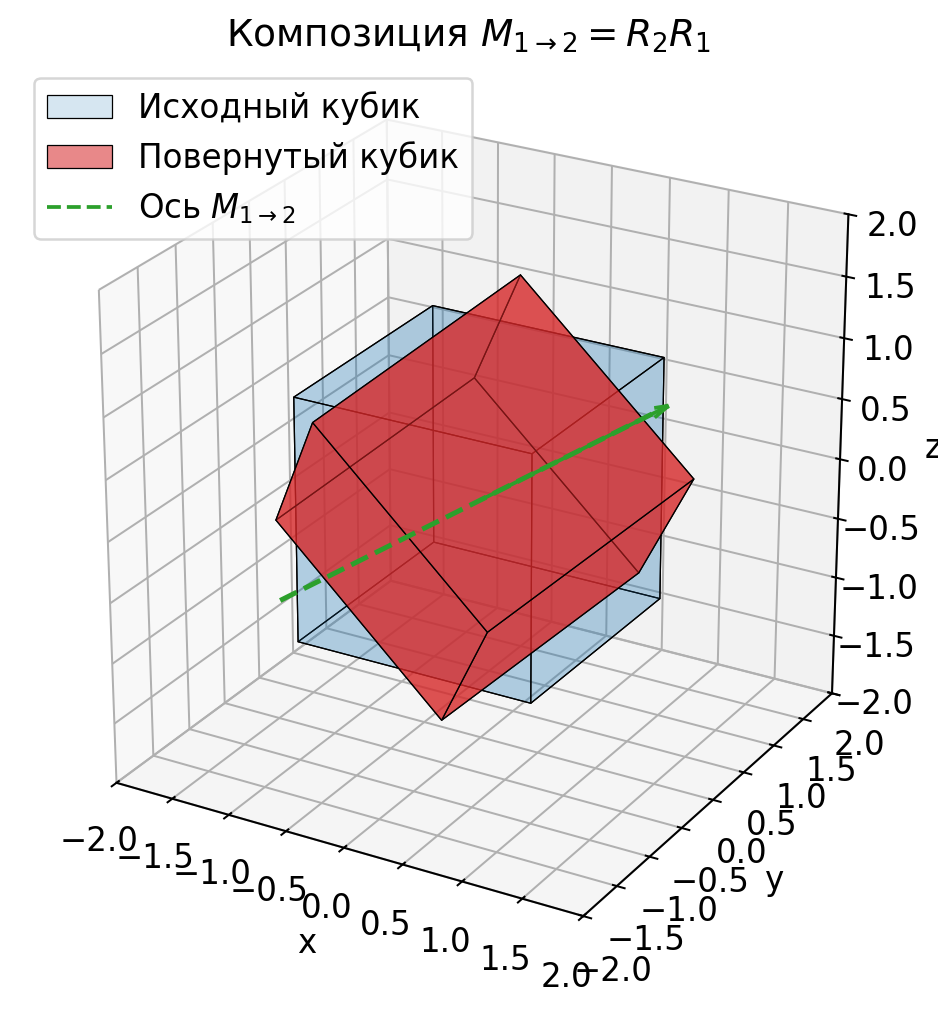
\includegraphics[width=0.66\linewidth]{figures/p4AB.png}
\caption{Композиция поворотов: сначала $R_1$, затем $R_2$}
\label{fig:p4AB}
\end{figure}


\begin{table}[H]\centering\singlespacing\small
\caption{Координаты вершин после применения $M_{1 \to 2}=R_2R_1$}
\label{tab:p4AB}
\begin{adjustbox}{max width=\linewidth}
\begin{tabular}{llll}
\toprule
№ вершины & $x$ & $y$ & $z$ \\
\midrule
1 & -0.674 & -1.265 & 0.972 \\
2 & -1.653 & -0.256 & -0.451 \\
3 & -0.899 & 1.460 & 0.247 \\
4 & 0.079 & 0.451 & 1.670 \\
5 & 0.899 & -1.460 & -0.247 \\
6 & -0.079 & -0.451 & -1.670 \\
7 & 0.674 & 1.265 & -0.972 \\
8 & 1.653 & 0.256 & 0.451 \\
\bottomrule\end{tabular}\end{adjustbox}\end{table}

\clearpage
\subsection*{Композиция $M_{2 \to 1}=R_1R_2$}

Порядок преобразований: сначала поворот вокруг оси $v_2$, затем поворот вокруг оси $v_1$. Эквивалентная ось вращения — $u_{2 \to 1}\approx(0.6774,\;0.5624,\;0.4741)^T$.

Результат показан на рисунке~\ref{fig:p4BA}, координаты вершин приведены в таблице~\ref{tab:p4BA}.

\begin{figure}[H]
\centering
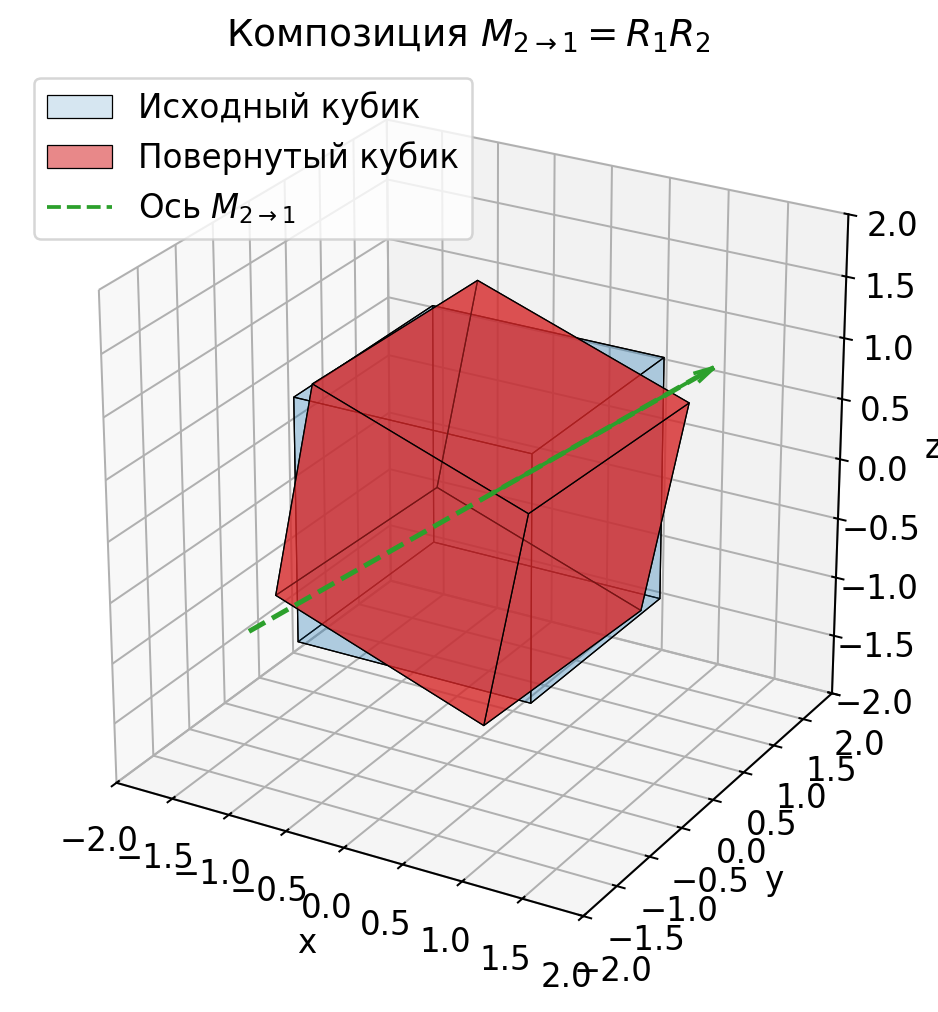
\includegraphics[width=0.66\linewidth]{figures/p4BA.png}
\caption{Композиция поворотов: сначала $R_2$, затем $R_1$}
\label{fig:p4BA}
\end{figure}


\begin{table}[H]\centering\singlespacing\small
\caption{Координаты вершин после применения $M_{2 \to 1}=R_1R_2$}
\label{tab:p4BA}
\begin{adjustbox}{max width=\linewidth}
\begin{tabular}{llll}
\toprule
№ вершины & $x$ & $y$ & $z$ \\
\midrule
1 & -1.330 & -0.782 & -0.787 \\
2 & -1.084 & 1.196 & -0.628 \\
3 & -0.593 & 0.980 & 1.299 \\
4 & -0.839 & -0.998 & 1.140 \\
5 & 0.593 & -0.980 & -1.299 \\
6 & 0.839 & 0.998 & -1.140 \\
7 & 1.330 & 0.782 & 0.787 \\
8 & 1.084 & -1.196 & 0.628 \\
\bottomrule\end{tabular}\end{adjustbox}\end{table}

\subsection*{Анализ полученных результатов}

\textbf{Влияние оси вращения.} Ось вращения определяет неподвижную прямую в пространстве: все точки, лежащие на ней, остаются на месте. Для оси $v_1$ это прямая

\begin{center}\adjustbox{max width=\linewidth}{$\displaystyle (0,0,0) + t(1,1,0),$}\end{center}

а для оси $v_2$ — прямая

\begin{center}\adjustbox{max width=\linewidth}{$\displaystyle (0,0,0) + t(0,1,1).$}\end{center}

Ось $v_1$ проходит через середины двух противоположных вертикальных ребер кубика, а ось $v_2$ — через середины двух противоположных ребер, параллельных оси $x$. Ни одна вершина кубика на этих осях не лежит, поэтому при выбранных углах вершины не остаются неподвижными.

\textbf{Влияние угла поворота.} Угол $\theta$ задает величину поворота вокруг выбранной оси:

\begin{itemize}
\item при $\theta=0$ кубик остается неподвижным;
\item при $\theta=\frac{\pi}{2}$ выполняется поворот на $90^\circ$;
\item при $\theta=\pi$ — поворот на $180^\circ$;
\item при $\theta=2\pi$ кубик возвращается в исходное положение.
\end{itemize}

При выбранных углах $90^\circ$ и $60^\circ$ кубик не переходит в себя, а занимает новое положение. При этом преобразование является движением: расстояния между вершинами сохраняются. Например, расстояние между вершинами 1 и 2 после применения $R_1$ остается равным 2.

\textbf{Влияние порядка преобразований.} Матрицы $M_{1 \to 2}=R_2R_1$ и $M_{2 \to 1}=R_1R_2$ различны, поэтому итоговая ориентация кубика зависит от порядка поворотов. При этом

\begin{center}\adjustbox{max width=\linewidth}{$\displaystyle M_{2 \to 1} = R_1M_{1 \to 2}R_1^{-1},$}\end{center}

то есть матрицы подобны. Угол поворота определяется следом верхнего левого блока $R$ размера $3\times3$:

\begin{center}\adjustbox{max width=\linewidth}{$\displaystyle \theta = \arccos\left(\frac{\operatorname{tr}R - 1}{2}\right).$}\end{center}

Для обеих матриц $\operatorname{tr}R \approx -0.241025$. Поскольку следы подобных матриц совпадают, у обеих композиций одинаковый угол поворота $128.35^\circ$, но эквивалентные оси различны:

\begin{center}\adjustbox{max width=\linewidth}{$\displaystyle u_{1 \to 2} \approx
\begin{bmatrix}
0.2847 \\
0.9552 \\
0.0813
\end{bmatrix},
\qquad
u_{2 \to 1} \approx
\begin{bmatrix}
0.6774 \\
0.5624 \\
0.4741
\end{bmatrix}.$}\end{center}

Таким образом, при одном и том же суммарном угле поворота кубик оказывается в разных положениях.

\textbf{Проверка корректности матриц поворота.} Для всех четырех матриц верхний блок $3 \times 3$ ортогонален:

\begin{center}\adjustbox{max width=\linewidth}{$\displaystyle R^T R = I,$}\end{center}

а его определитель равен единице:

\begin{center}\adjustbox{max width=\linewidth}{$\displaystyle \det R = 1.$}\end{center}

Это означает, что преобразования сохраняют длины, углы, объемы и ориентацию пространства. Кроме того, для осей выполняются равенства

\begin{center}\adjustbox{max width=\linewidth}{$\displaystyle R_1
\begin{bmatrix}
1 \\
1 \\
0 \\
0
\end{bmatrix}
=
\begin{bmatrix}
1 \\
1 \\
0 \\
0
\end{bmatrix},
\qquad
R_2
\begin{bmatrix}
0 \\
1 \\
1 \\
0
\end{bmatrix}
=
\begin{bmatrix}
0 \\
1 \\
1 \\
0
\end{bmatrix}.$}\end{center}

Здесь направления осей записаны в однородных координатах с нулевой четвертой компонентой. Следовательно, векторы $v_1$ и $v_2$ действительно являются собственными векторами соответствующих матриц с собственным числом 1, то есть задают оси вращения.

\subsection*{Восстановление оси вращения по матрице поворота}

Для композиции поворотов эквивалентную ось можно восстановить непосредственно из матрицы. Если

\begin{center}\adjustbox{max width=\linewidth}{$\displaystyle R =
\begin{bmatrix}
r_{11} & r_{12} & r_{13} \\
r_{21} & r_{22} & r_{23} \\
r_{31} & r_{32} & r_{33}
\end{bmatrix},$}\end{center}

то вектор оси вращения пропорционален вектору

\begin{center}\adjustbox{max width=\linewidth}{$\displaystyle u \sim
\begin{bmatrix}
r_{32} - r_{23} \\
r_{13} - r_{31} \\
r_{21} - r_{12}
\end{bmatrix}.$}\end{center}

После нормировки

\begin{center}\adjustbox{max width=\linewidth}{$\displaystyle u = \frac{u}{\|u\|}.$}\end{center}

Именно так в программе получены оси $u_{1 \to 2}$ и $u_{2 \to 1}$. Формула применима при $\sin\theta \neq 0$; для углов $0$ и $\pi$ вектор оси находится через собственный вектор матрицы $R$ с собственным числом 1.

\par\noindent\begin{minipage}{\linewidth}
\subsection*{Вывод по заданию 4}

В задании построена матрица поворота вокруг произвольной оси, проходящей через центр кубика. Матричная экспонента $e^{J\theta}$ сведена к формуле Родригеса, а для осей $x$, $y$ и $z$ получены частные случаи $R_x$, $R_y$, $R_z$.

Для двух выбранных осей и углов построены матрицы $R_1$ и $R_2$, а также две их композиции — $R_2R_1$ и $R_1R_2$. Расчеты и результаты программы показывают, что матрицы композиций различны: при одинаковом угле $128.35^\circ$ оси вращения не совпадают. Следовательно, порядок применения поворотов влияет на итоговую ориентацию кубика.

Корректность матриц подтверждена проверками: $R^TR=I$, $\det R=1$, а векторы $v_1$ и $v_2$ остаются неподвижными. На всех графиках дополнительно показан вектор, коллинеарный оси вращения.

\end{minipage}\par
\section{Задание 5. Вращение кубика вокруг вершины}

\subsection*{Общая формула поворота вокруг оси, проходящей через точку}

Пусть ось вращения проходит через точку

\begin{center}\adjustbox{max width=\linewidth}{$\displaystyle M =
\begin{bmatrix}
x_0 \\
y_0 \\
z_0
\end{bmatrix}$}\end{center}

и имеет направление $v$, а угол поворота равен $\theta$. Чтобы свести такое вращение к уже известному повороту вокруг начала координат, выполним три аффинных преобразования.

1. Перенесем объект так, чтобы точка $M$ совпала с началом координат:

\begin{center}\adjustbox{max width=\linewidth}{$\displaystyle T(-M) =
\begin{bmatrix}
1 & 0 & 0 & -x_0 \\
0 & 1 & 0 & -y_0 \\
0 & 0 & 1 & -z_0 \\
0 & 0 & 0 & 1
\end{bmatrix}.$}\end{center}

2. Повернем объект вокруг начала координат вокруг оси с направлением $v$ на угол $\theta$:

\begin{center}\adjustbox{max width=\linewidth}{$\displaystyle R_v(\theta).$}\end{center}

3. Вернем точку $M$ на место обратным переносом:

\begin{center}\adjustbox{max width=\linewidth}{$\displaystyle T(M) =
\begin{bmatrix}
1 & 0 & 0 & x_0 \\
0 & 1 & 0 & y_0 \\
0 & 0 & 1 & z_0 \\
0 & 0 & 0 & 1
\end{bmatrix}.$}\end{center}

Итоговая матрица преобразования имеет вид

\begin{center}\adjustbox{max width=\linewidth}{$\displaystyle M_{\text{pivot}} = T(M)\,R_v(\theta)\,T(-M).$}\end{center}

Обозначим через $R$ верхний левый блок $3 \times 3$ матрицы $R_v(\theta)$. Тогда

\begin{center}\adjustbox{max width=\linewidth}{$\displaystyle M_{\text{pivot}} =
\begin{bmatrix}
R & M - RM \\
\mathbf{0}_{1 \times 3} & 1
\end{bmatrix}.$}\end{center}

Действительно,

\begin{center}\adjustbox{max width=\linewidth}{$\displaystyle T(M)
\begin{bmatrix}
R & 0 \\
\mathbf{0}_{1 \times 3} & 1
\end{bmatrix}
T(-M)
=
\begin{bmatrix}
R & M - RM \\
\mathbf{0}_{1 \times 3} & 1
\end{bmatrix}.$}\end{center}

Вектор $M - RM$ — это сдвиг, который компенсирует поворот точки $M$ вокруг начала координат. Поэтому

\begin{center}\adjustbox{max width=\linewidth}{$\displaystyle M_{\text{pivot}}
\begin{bmatrix}
M \\
1
\end{bmatrix}
=
\begin{bmatrix}
M \\
1
\end{bmatrix},$}\end{center}

то есть выбранная точка оси остается неподвижной. Матрица $R$ — это матрица поворота вокруг начала координат, построенная в задании 4.

\subsection*{Выбранная матрица преобразования}

Выберем вершину кубика

\begin{center}\adjustbox{max width=\linewidth}{$\displaystyle M =
\begin{bmatrix}
1 \\
1 \\
1
\end{bmatrix}.$}\end{center}

В однородных координатах:

\begin{center}\adjustbox{max width=\linewidth}{$\displaystyle M =
\begin{bmatrix}
1 \\
1 \\
1 \\
1
\end{bmatrix}.$}\end{center}

Ось вращения зададим направлением

\begin{center}\adjustbox{max width=\linewidth}{$\displaystyle v =
\begin{bmatrix}
1 \\
1 \\
0
\end{bmatrix},
\qquad
\theta = \frac{\pi}{2},
\qquad
u =
\frac{v}{\|v\|}
=
\begin{bmatrix}
\frac{1}{\sqrt{2}} \\
\frac{1}{\sqrt{2}} \\
0
\end{bmatrix}.$}\end{center}

Ось проходит через вершину $M$ и описывается уравнением

\begin{center}\adjustbox{max width=\linewidth}{$\displaystyle L(t) = M + tu
=
\begin{bmatrix}
1 \\
1 \\
1
\end{bmatrix}
+
t
\begin{bmatrix}
\frac{1}{\sqrt{2}} \\
\frac{1}{\sqrt{2}} \\
0
\end{bmatrix}.$}\end{center}

Матрица поворота вокруг этой оси на угол $\theta=\frac{\pi}{2}$:

\begin{center}\adjustbox{max width=\linewidth}{$\displaystyle R_v\left(\frac{\pi}{2}\right) =
\begin{bmatrix}
\frac{1}{2} & \frac{1}{2} & \frac{1}{\sqrt{2}} & 0 \\
\frac{1}{2} & \frac{1}{2} & -\frac{1}{\sqrt{2}} & 0 \\
-\frac{1}{\sqrt{2}} & \frac{1}{\sqrt{2}} & 0 & 0 \\
0 & 0 & 0 & 1
\end{bmatrix}.$}\end{center}

Матрицы переносов:

\begin{center}\adjustbox{max width=\linewidth}{$\displaystyle T(-M) =
\begin{bmatrix}
1 & 0 & 0 & -1 \\
0 & 1 & 0 & -1 \\
0 & 0 & 1 & -1 \\
0 & 0 & 0 & 1
\end{bmatrix},
\qquad
T(M) =
\begin{bmatrix}
1 & 0 & 0 & 1 \\
0 & 1 & 0 & 1 \\
0 & 0 & 1 & 1 \\
0 & 0 & 0 & 1
\end{bmatrix}.$}\end{center}

После перемножения получаем

\begin{center}\adjustbox{max width=\linewidth}{$\displaystyle \begin{gathered}
M_{\text{pivot}} = T(M)\,R_v\left(\frac{\pi}{2}\right)\,T(-M)
=
\begin{bmatrix}
\frac{1}{2} & \frac{1}{2} & \frac{1}{\sqrt{2}} & -\frac{1}{\sqrt{2}} \\
\frac{1}{2} & \frac{1}{2} & -\frac{1}{\sqrt{2}} & \frac{1}{\sqrt{2}} \\
-\frac{1}{\sqrt{2}} & \frac{1}{\sqrt{2}} & 0 & 1 \\
0 & 0 & 0 & 1
\end{bmatrix} \\[4pt]
\approx \begin{bmatrix}
0.500000 & 0.500000 & 0.707107 & -0.707107 \\
0.500000 & 0.500000 & -0.707107 & 0.707107 \\
-0.707107 & 0.707107 & 0.000000 & 1.000000 \\
0 & 0 & 0 & 1
\end{bmatrix}.
\end{gathered}$}\end{center}

Проверим неподвижность выбранной вершины:

\begin{center}\adjustbox{max width=\linewidth}{$\displaystyle M_{\text{pivot}}
\begin{bmatrix}
1 \\
1 \\
1 \\
1
\end{bmatrix}
=
\begin{bmatrix}
1 \\
1 \\
1 \\
1
\end{bmatrix}.$}\end{center}

Следовательно, вершина $M=(1,1,1)$ остается на месте. На той же прямой лежит вершина $(-1,-1,1)$, поэтому она также неподвижна.

\subsection*{Результаты выполнения программы}

На рисунке~\ref{fig:p5} показаны исходный кубик (синий, полупрозрачный), кубик после применения $M_{\text{pivot}}$ (красный) и ось вращения, проходящая через вершину $M=(1,1,1)$.

\begin{figure}[H]
\centering
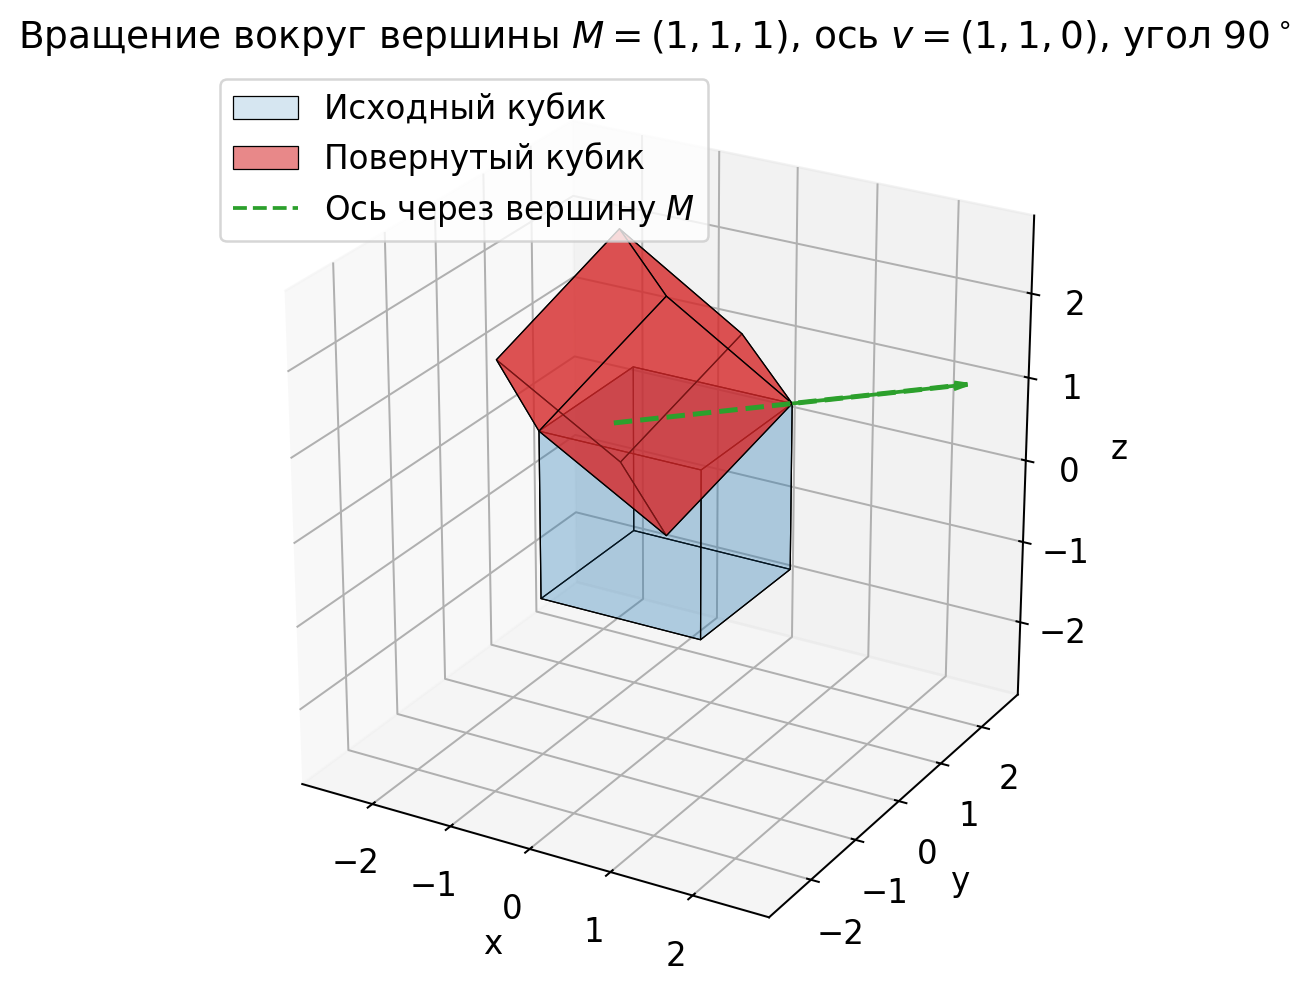
\includegraphics[width=0.72\linewidth]{figures/p5.png}
\caption{Поворот вокруг оси через вершину $M=(1,1,1)$}
\label{fig:p5}
\end{figure}


\begin{table}[H]\centering\singlespacing\small
\caption{Координаты вершин после применения $M_{\text{pivot}}$}
\label{tab:p5}
\begin{adjustbox}{max width=\linewidth}
\begin{tabular}{llll}
\toprule
№ вершины & $x$ & $y$ & $z$ \\
\midrule
1 & -2.414 & 0.414 & 1.000 \\
2 & -1.414 & 1.414 & -0.414 \\
3 & -0.414 & 2.414 & 1.000 \\
4 & -1.414 & 1.414 & 2.414 \\
5 & -1.000 & -1.000 & 1.000 \\
6 & 0.000 & 0.000 & -0.414 \\
7 & 1.000 & 1.000 & 1.000 \\
8 & 0.000 & 0.000 & 2.414 \\
\bottomrule\end{tabular}\end{adjustbox}\end{table}

Верхний блок матрицы ортогонален: $R^TR=I$, а его определитель равен единице: $\det R=1$. Четвертая однородная координата всех вершин остается равной единице, поэтому преобразование является аффинным. Вершины 5 и 7 не меняют положения, поскольку лежат на оси вращения.

\par\noindent\begin{minipage}{\linewidth}
\subsection*{Вывод по заданию 5}

Получена общая формула матрицы поворота вокруг оси с направлением $v$, проходящей через точку $M(x_0,y_0,z_0)$:

\begin{center}\adjustbox{max width=\linewidth}{$\displaystyle M_{\text{pivot}} = T(M)\,R_v(\theta)\,T(-M).$}\end{center}

Для вершины $M=(1,1,1)$, оси $v=(1,1,0)$ и угла $\theta=\frac{\pi}{2}$ построена конкретная матрица $M_{\text{pivot}}$. Она переводит кубик в новое положение, оставляя выбранную вершину неподвижной. Результат подтвержден графиком и координатами вершин: преобразование является движением, а ось вращения проходит через вершину кубика.
\end{minipage}\par
\clearpage
\unnumsection{Заключение по заданиям 1--5}
Однородные координаты позволяют задавать масштабирование и перенос матрицами
одного размера $4\times4$. Композиция выбранных масштабов восстанавливает
размеры по $x$ и $z$, сохраняя растяжение по $y$. Два переноса складываются,
а порядок переноса и масштабирования влияет на положение образа:
в $ST$ масштабируется и смещение. Равенство определителей $TS$ и $ST$
показывает одинаковое изменение объёма, но не равенство преобразований.
Повороты, вычисленные с помощью матричной экспоненты,
сохраняют расстояния, углы и объём. Перестановка двух поворотов меняет
эквивалентную ось, хотя угол в рассмотренном случае совпадает.
Композиция $T(M)R_v(\theta)T(-M)$ позволяет вращать фигуру вокруг оси
через заданную точку, сохраняя точки этой оси неподвижными.
\clearpage
\unnumsection{Приложение А. Код блока A}
\begingroup\setstretch{0.95}
\VerbatimInput[breaklines,fontsize=\footnotesize,numbers=left,
numbersep=8pt,xleftmargin=14pt,frame=single]{../code/block_a.py}
\captionof{lstlisting}{Отрисовка фигур, масштабирование и перенос куба}
\endgroup
\clearpage
\unnumsection{Приложение Б. Код заданий 4--5}
\begingroup\setstretch{0.95}
\VerbatimInput[breaklines,fontsize=\footnotesize,numbers=left,
numbersep=8pt,xleftmargin=14pt,frame=single]{../block_45.py}
\captionof{lstlisting}{Повороты вокруг оси через центр куба и через его вершину}
\endgroup
\end{document}
